\newcommand{\End}{\ensuremath{\mathrm{End}}}
\newcommand{\Hom}{\ensuremath{\mathrm{Hom}}}

\newcommand{\arbreoptrois}{
\begin{tikzpicture}[scale=0.15,baseline=(pt_base.base)]

\coordinate (pt_base) at (0,-0.5) ;

\draw (0,1.25) -- (0,0) ;
\draw (-1.25,1.25) -- (0,0) ;
\draw (1.25,1.25) -- (0,0) ;
\draw (0,-1.25) -- (0,0) ;

\end{tikzpicture}
}

\newcommand{\premiertermecobarbarA}{
\begin{tikzpicture}[scale=0.15,baseline=(pt_base.base)]

\coordinate (pt_base) at (0,-0.5) ;

\draw (-1.25,1.25) -- (0,0) ;
\draw (1.25,1.25) -- (0,0) ;
\draw (0,-1.25) -- (0,0) ;

\end{tikzpicture}
}

\newcommand{\premiertermecobarbarAprime}{
\begin{tikzpicture}[scale=0.07,baseline=(pt_base.base)]

\coordinate (pt_base) at (0,-0.5) ;

\draw (-1.25,1.25) -- (0,0) ;
\draw (1.25,1.25) -- (0,0) ;
\draw (0,-1.25) -- (0,0) ;

\end{tikzpicture}
}

\newcommand{\premiertermecobarbarB}{
\begin{tikzpicture}[scale = 0.15,baseline = (O.base)]
\node (K) at (-0.625,0.625) {} ;
\node (L) at (0,0) {} ;
\draw (-0.625,0.625) -- (0,1.25) ;
\draw (-1.25,1.25) -- (0,0) ;
\draw (1.25,1.25) -- (0,0) ;
\draw (0,-1.25) -- (0,0) ;
\node (O) at (0,-0.5) {} ;
\end{tikzpicture}
}

\newcommand{\premiertermecobarbarC}{
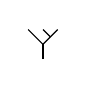
\begin{tikzpicture}[scale = 0.15,baseline = (O.base)]
\node (K) at (0.625,0.625) {} ;
\node (L) at (0,0) {} ;
\draw (0.625,0.625) -- (0,1.25) ;
\draw (-1.25,1.25) -- (0,0) ;
\draw (1.25,1.25) -- (0,0) ;
\draw (0,-1.25) -- (0,0) ;
\node (O) at (0,-0.5) {} ;
\end{tikzpicture}
}

\newcommand{\premiertermecobarbarD}{
\begin{tikzpicture}[scale=0.15,baseline=(pt_base.base)]

\coordinate (pt_base) at (0,-0.5) ;

\draw (0,1.25) -- (0,0) ;
\draw (-1.25,1.25) -- (0,0) ;
\draw (1.25,1.25) -- (0,0) ;
\draw (0,-1.25) -- (0,0) ;

\end{tikzpicture}
}

\newcommand{\arbreopdeuxcol}[1]{
\begin{tikzpicture}[scale=0.15,baseline=(pt_base.base)]

\coordinate (pt_base) at (0,-0.5) ;

\draw[#1] (-1.25,1.25) -- (0,0) ;
\draw[#1] (1.25,1.25) -- (0,0) ;
\draw[#1] (0,-1.25) -- (0,0) ;

\end{tikzpicture}
}

% Opération ternaire colorée de l'opérade A-infini

\newcommand{\arbreoptroiscol}[1]{
\begin{tikzpicture}[scale=0.15,baseline=(pt_base.base)]

\coordinate (pt_base) at (0,-0.5) ;

\draw[#1] (0,1.25) -- (0,0) ;
\draw[#1] (-1.25,1.25) -- (0,0) ;
\draw[#1] (1.25,1.25) -- (0,0) ;
\draw[#1] (0,-1.25) -- (0,0) ;

\end{tikzpicture}
}

\usetikzlibrary{decorations.pathreplacing,calligraphy}
\usetikzlibrary{decorations.pathmorphing}

\newcommand{\compositionlabelIJ}{
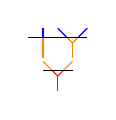
\begin{tikzpicture}[scale=0.15,baseline=(pt_base.base)]

\coordinate (pt_base) at (0,-0.5) ;

\draw[orange] (-1.25,1.25) -- (-0.5,0.5) ;
\draw[orange] (1.25,1.25) -- (0.5,0.5) ;

\draw[red] (-0.5,0.5) -- (0,0) ;
\draw[red] (0.5,0.5) -- (0,0) ;
\draw[red] (0,-1.25) -- (0,0) ;

\draw (-1.25,0.5) -- (1.25,0.5) ;

\begin{scope}[xshift=1.25cm,yshift=2.8cm]

\draw[blue] (-1.25,1.25) -- (-0.5,0.5) ;
\draw[blue] (1.25,1.25) -- (0.5,0.5) ;

\draw[orange] (-0.5,0.5) -- (0,0) ;
\draw[orange] (0.5,0.5) -- (0,0) ;
\draw[orange] (0,-1.25) -- (0,0) ;

\draw (-1.25,0.5) -- (1.25,0.5) ;

\end{scope}

\begin{scope}[xshift=-1.25cm,yshift=2.8cm]

\draw[blue] (0,1.25) -- (0,0.5) ;
\draw[orange] (0,-1.25) -- (0,0.5) ;

\draw (-1.25,0.5) -- (1.25,0.5) ;

\end{scope}

\end{tikzpicture}
}

\newcommand{\compositionlabelKL}{
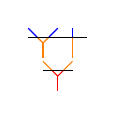
\begin{tikzpicture}[scale=0.15,baseline=(pt_base.base)]

\coordinate (pt_base) at (0,-0.5) ;

\draw[orange] (-1.25,1.25) -- (-0.5,0.5) ;
\draw[orange] (1.25,1.25) -- (0.5,0.5) ;

\draw[red] (-0.5,0.5) -- (0,0) ;
\draw[red] (0.5,0.5) -- (0,0) ;
\draw[red] (0,-1.25) -- (0,0) ;

\draw (-1.25,0.5) -- (1.25,0.5) ;

\begin{scope}[xshift=-1.25cm,yshift=2.8cm]

\draw[blue] (-1.25,1.25) -- (-0.5,0.5) ;
\draw[blue] (1.25,1.25) -- (0.5,0.5) ;

\draw[orange] (-0.5,0.5) -- (0,0) ;
\draw[orange] (0.5,0.5) -- (0,0) ;
\draw[orange] (0,-1.25) -- (0,0) ;

\draw (-1.25,0.5) -- (1.25,0.5) ;

\end{scope}

\begin{scope}[xshift=1.25cm,yshift=2.8cm]

\draw[blue] (0,1.25) -- (0,0.5) ;
\draw[orange] (0,-1.25) -- (0,0.5) ;

\draw (-1.25,0.5) -- (1.25,0.5) ;

\end{scope}

\end{tikzpicture}
}

\newcommand{\compositionlabelJK}{
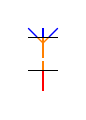
\begin{tikzpicture}[scale=0.15,baseline=(pt_base.base)]

\coordinate (pt_base) at (0,-0.5) ;

\draw[blue] (0,1.25) -- (0,0.5) ;
\draw[blue] (-1.25,1.25) -- (-0.5,0.5) ;
\draw[blue] (1.25,1.25) -- (0.5,0.5) ;

\draw[orange] (0,0.5) -- (0,0) ;
\draw[orange] (-0.5,0.5) -- (0,0) ;
\draw[orange] (0.5,0.5) -- (0,0) ;
\draw[orange] (0,-1.25) -- (0,0) ;

\draw (-1.25,0.5) -- (1.25,0.5) ;

\begin{scope}[yshift = -2.8cm ]

\draw[orange] (0,1.25) -- (0,0.5) ;
\draw[red] (0,-1.25) -- (0,0.5) ;

\draw (-1.25,0.5) -- (1.25,0.5) ;

\end{scope}

\end{tikzpicture}
}

\newcommand{\compositionlabelIL}{
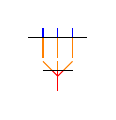
\begin{tikzpicture}[scale=0.15,baseline=(pt_base.base)]

\coordinate (pt_base) at (0,-0.5) ;

\draw[orange] (0,1.25) -- (0,0.5) ;
\draw[orange] (-1.25,1.25) -- (-0.5,0.5) ;
\draw[orange] (1.25,1.25) -- (0.5,0.5) ;

\draw[red] (0,0.5) -- (0,0) ;
\draw[red] (-0.5,0.5) -- (0,0) ;
\draw[red] (0.5,0.5) -- (0,0) ;
\draw[red] (0,-1.25) -- (0,0) ;

\draw (-1.25,0.5) -- (1.25,0.5) ;

\begin{scope}[yshift = 2.8cm ]

\draw[blue] (0,1.25) -- (0,0.5) ;
\draw[orange] (0,-1.25) -- (0,0.5) ;

\draw (-1.25,0.5) -- (1.25,0.5) ;

\end{scope}

\begin{scope}[xshift= -1.25cm, yshift = 2.8cm ]

\draw[blue] (0,1.25) -- (0,0.5) ;
\draw[orange] (0,-1.25) -- (0,0.5) ;

\draw (-1.25,0.5) -- (1.25,0.5) ;

\end{scope}

\begin{scope}[xshift= 1.25cm, yshift = 2.8cm ]

\draw[blue] (0,1.25) -- (0,0.5) ;
\draw[orange] (0,-1.25) -- (0,0.5) ;

\draw (-1.25,0.5) -- (1.25,0.5) ;

\end{scope}

\end{tikzpicture}
}

% Opérations colorées de l'opérade A-infini

\newcommand{\arbreoprouge}[1]{
\begin{tikzpicture}[scale=#1,baseline=(pt_base.base)]

\coordinate (pt_base) at (0,-0.5) ;

\draw[red] (-2,1.25) -- (0,0) ;
\draw[red] (-1,1.25) -- (0,0) ;
\draw[red] (1,1.25) -- (0,0) ;
\draw[red] (2,1.25) -- (0,0) ;
\draw[red] (0,-1.25) -- (0,0) ;

\draw[red] [densely dotted] (-0.5,0.9) -- (0.5,0.9) ;

\end{tikzpicture}}

\newcommand{\arbreopbleu}[1]{
\begin{tikzpicture}[scale=#1,baseline=(pt_base.base)]

\coordinate (pt_base) at (0,-0.5) ;

\draw[blue] (-2,1.25) -- (0,0) ;
\draw[blue] (-1,1.25) -- (0,0) ;
\draw[blue] (1,1.25) -- (0,0) ;
\draw[blue] (2,1.25) -- (0,0) ;
\draw[blue] (0,-1.25) -- (0,0) ;

\draw[blue] [densely dotted] (-0.5,0.9) -- (0.5,0.9) ;

\end{tikzpicture}}

% Opérations du bimodule opéradique A-infini - Morph

\newcommand{\arbreopmorph}[1]{
\begin{tikzpicture}[scale=#1,baseline=(pt_base.base)]

\coordinate (pt_base) at (0,-0.5) ;

\draw[blue] (-2,1.25) -- (0,0) ;
\draw[blue] (-1,1.25) -- (0,0) ;
\draw[blue] (1,1.25) -- (0,0) ;
\draw[blue] (2,1.25) -- (0,0) ;

\draw[red] (0,-1.25) -- (0,0) ;

\draw[blue] [densely dotted] (-0.5,0.9) -- (0.5,0.9) ;

\draw  (-1.5,0) -- (1.5,0) ;

\end{tikzpicture}}

\newcommand{\arbreopmorphcompun}{
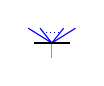
\begin{tikzpicture}[scale=0.15,baseline=(pt_base.base)]

\coordinate (pt_base) at (0,-0.5) ;

\draw[blue] (-2,1.25) -- (0,0) ;
\draw[blue] (-1,1.25) -- (0,0) ;
\draw[blue] (1,1.25) -- (0,0) ;
\draw[blue] (2,1.25) -- (0,0) ;

\draw[orange] (0,-1.25) -- (0,0) ;

\draw[blue] [densely dotted] (-0.5,0.9) -- (0.5,0.9) ;

\draw  (-1.5,0) -- (1.5,0) ;

\end{tikzpicture}}

\newcommand{\arbreopmorphcompdeux}{
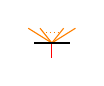
\begin{tikzpicture}[scale=0.15,baseline=(pt_base.base)]

\coordinate (pt_base) at (0,-0.5) ;

\draw[orange] (-2,1.25) -- (0,0) ;
\draw[orange] (-1,1.25) -- (0,0) ;
\draw[orange] (1,1.25) -- (0,0) ;
\draw[orange] (2,1.25) -- (0,0) ;

\draw[red] (0,-1.25) -- (0,0) ;

\draw[orange] [densely dotted] (-0.5,0.9) -- (0.5,0.9) ;

\draw  (-1.5,0) -- (1.5,0) ;

\end{tikzpicture}}

% Opération binaire de A-infini - Morph

\newcommand{\arbreopdeuxmorph}{
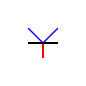
\begin{tikzpicture}[scale=0.15,baseline=(pt_base.base)]

\coordinate (pt_base) at (0,-0.5) ;

\draw[blue] (-1.25,1.25) -- (0,0) ;
\draw[blue] (1.25,1.25) -- (0,0) ;
\draw[red] (0,-1.25) -- (0,0) ;

\draw (-1.25,0) -- (1.25,0) ;

\end{tikzpicture}
}

\newcommand{\arbreopdeuxmorphcompun}{
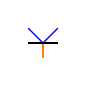
\begin{tikzpicture}[scale=0.15,baseline=(pt_base.base)]

\coordinate (pt_base) at (0,-0.5) ;

\draw[blue] (-1.25,1.25) -- (0,0) ;
\draw[blue] (1.25,1.25) -- (0,0) ;
\draw[orange] (0,-1.25) -- (0,0) ;

\draw (-1.25,0) -- (1.25,0) ;

\end{tikzpicture}
}

\newcommand{\arbreopdeuxmorphcompdeux}{
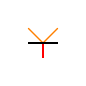
\begin{tikzpicture}[scale=0.15,baseline=(pt_base.base)]

\coordinate (pt_base) at (0,-0.5) ;

\draw[orange] (-1.25,1.25) -- (0,0) ;
\draw[orange] (1.25,1.25) -- (0,0) ;
\draw[red] (0,-1.25) -- (0,0) ;

\draw (-1.25,0) -- (1.25,0) ;

\end{tikzpicture}
}

\newcommand{\arbreopcompun}{
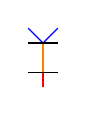
\begin{tikzpicture}[scale=0.15,baseline=(pt_base.base)]

\coordinate (pt_base) at (0,-2) ;

\draw[blue] (-1.25,1.25) -- (0,0) ;
\draw[blue] (1.25,1.25) -- (0,0) ;
\draw[orange] (0,-2.5) -- (0,0) ;
\draw[red] (0,-3.75) -- (0,-2.5) ;

\draw (-1.25,0) -- (1.25,0) ;

\draw (-1.25,-2.5) -- (1.25,-2.5) ;

\end{tikzpicture}
}

\newcommand{\arbreopcompdeux}{
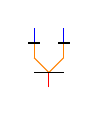
\begin{tikzpicture}[scale=0.15,baseline=(pt_base.base)]

\coordinate (pt_base) at (0,0.5) ;

\draw[blue] (-1.25,3.75) -- (-1.25,2.5) ;
\draw[blue] (1.25,3.75) -- (1.25,2.5) ;
\draw[orange] (-1.25,1.25) -- (-1.25,2.5) ;
\draw[orange] (1.25,1.25) -- (1.25,2.5) ;
\draw[orange] (-1.25,1.25) -- (0,0) ;
\draw[orange] (1.25,1.25) -- (0,0) ;
\draw[red] (0,-1.25) -- (0,0) ;

\draw (-1.25,0) -- (1.25,0) ;
\draw (-1.75,2.5) -- (-0.75,2.5) ;
\draw (1.75,2.5) -- (0.75,2.5) ;

\end{tikzpicture}
}

% Opération ternaire de A-infini - Morph

\newcommand{\arbreoptroismorph}{
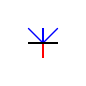
\begin{tikzpicture}[scale=0.15,baseline=(pt_base.base)]

\coordinate (pt_base) at (0,-0.5) ;

\draw[blue] (0,1.25) -- (0,0) ;
\draw[blue] (-1.25,1.25) -- (0,0) ;
\draw[blue] (1.25,1.25) -- (0,0) ;

\draw[red] (0,-1.25) -- (0,0) ;

\draw (-1.25,0) -- (1.25,0) ;

\end{tikzpicture}
}

\newcommand{\arbreoptroismorphcompun}{
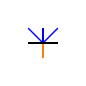
\begin{tikzpicture}[scale=0.15,baseline=(pt_base.base)]

\coordinate (pt_base) at (0,-0.5) ;

\draw[blue] (0,1.25) -- (0,0) ;
\draw[blue] (-1.25,1.25) -- (0,0) ;
\draw[blue] (1.25,1.25) -- (0,0) ;

\draw[orange] (0,-1.25) -- (0,0) ;

\draw (-1.25,0) -- (1.25,0) ;

\end{tikzpicture}
}

\newcommand{\arbreoptroismorphcompdeux}{
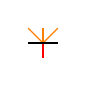
\begin{tikzpicture}[scale=0.15,baseline=(pt_base.base)]

\coordinate (pt_base) at (0,-0.5) ;

\draw[orange] (0,1.25) -- (0,0) ;
\draw[orange] (-1.25,1.25) -- (0,0) ;
\draw[orange] (1.25,1.25) -- (0,0) ;

\draw[red] (0,-1.25) -- (0,0) ;

\draw (-1.25,0) -- (1.25,0) ;

\end{tikzpicture}
}

% Opération quaternaire de A-infini - Morph

\newcommand{\arbreopquatremorph}{
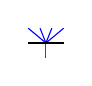
\begin{tikzpicture}[scale=0.15,baseline=(pt_base.base)]

\coordinate (pt_base) at (0,-0.5) ;

\draw[blue] (-1.5,1.25) -- (0,0) ;
\draw[blue] (1.5,1.25) -- (0,0) ;
\draw[blue] (-0.5,1.25) -- (0,0) ;
\draw[blue] (0.5,1.25) -- (0,0) ;

\draw[red] (0,-1.25) -- (0,0) ;

\draw (-1.5,0) -- (1.5,0) ;

\end{tikzpicture}
}

\newcommand{\arbreopquatremorphcompun}{
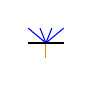
\begin{tikzpicture}[scale=0.15,baseline=(pt_base.base)]

\coordinate (pt_base) at (0,-0.5) ;

\draw[blue] (-1.5,1.25) -- (0,0) ;
\draw[blue] (1.5,1.25) -- (0,0) ;
\draw[blue] (-0.5,1.25) -- (0,0) ;
\draw[blue] (0.5,1.25) -- (0,0) ;

\draw[orange] (0,-1.25) -- (0,0) ;

\draw (-1.5,0) -- (1.5,0) ;

\end{tikzpicture}
}

\newcommand{\arbreopquatremorphcompdeux}{

\begin{tikzpicture}[scale=0.15,baseline=(pt_base.base)]

\coordinate (pt_base) at (0,-0.5) ;

\draw[orange] (-1.5,1.25) -- (0,0) ;
\draw[orange] (1.5,1.25) -- (0,0) ;
\draw[orange] (-0.5,1.25) -- (0,0) ;
\draw[orange] (0.5,1.25) -- (0,0) ;

\draw[red] (0,-1.25) -- (0,0) ;

\draw (-1.5,0) -- (1.5,0) ;

\end{tikzpicture}
}

% Compositions partielles de A-infini - Morph 1

\newcommand{\eqainfmorphun}{
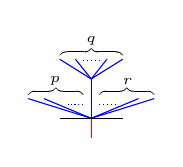
\begin{tikzpicture}[scale=0.2,baseline=(pt_base.base)]

\coordinate (pt_base) at (0,1.25) ;

%étiquetages

\draw [decorate,    decoration = {calligraphic brace}] (-4,1.5) --  (-0.5,1.5) ;
\draw [decorate,    decoration = {calligraphic brace}] (0.5,1.5) --  (4,1.5) ;
\draw [decorate,    decoration = {calligraphic brace}] (-2,4) --  (2,4) ;

\node[above] at (-2.3,1.5) {\tiny $p$} ; 
\node[above] at (0,4) {\tiny $q$} ; 
\node[above] at (2.3,1.5) {\tiny $r$} ; 

% traits bicolorés

\draw[blue] (-4,1.25) -- (0,0) ;
\draw[blue] (-3,1.25) -- (0,0) ;
\draw[blue] (4,1.25) -- (0,0) ;
\draw[blue] (3,1.25) -- (0,0) ;
\draw[blue] (0,1.25) -- (0,0) ;

\draw[red] (0,-1.25) -- (0,0) ; 

% traits arbre supérieur

\draw[blue] (-2,3.75) -- (0,2.5) ;
\draw[blue] (-1,3.75) -- (0,2.5) ;
\draw[blue] (1,3.75) -- (0,2.5) ;
\draw[blue] (2,3.75) -- (0,2.5) ;
\draw[blue] (0,1.25) -- (0,2.5) ;

% autres traits

\draw[blue] [densely dotted] (-0.5,3.65) -- (0.5,3.65) ;
\draw[blue] [densely dotted] (-0.5,0.9) -- (-1.5,0.9) ;
\draw[blue] [densely dotted] (0.5,0.9) -- (1.5,0.9) ;

\draw (-2,0) -- (2,0) ;

\end{tikzpicture}}

% Compositions partielles de A-infini - Morph 2

\newcommand{\compainf}{
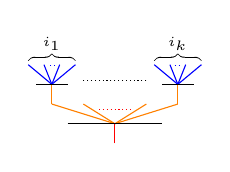
\begin{tikzpicture}[scale=0.2,baseline=(pt_base.base)]

\coordinate (pt_base) at (0,1.25) ;

% étiquettes 

\draw [decorate,    decoration = {calligraphic brace}] (-5.5,4) --  (-2.5,4) ;
\draw [decorate,    decoration = {calligraphic brace}] (2.5,4) --  (5.5,4) ;

\node[above] at (-4,4) {\tiny $i_1$} ; 
\node[above] at (4,4) {\tiny $i_k$} ; 


% arbre inférieur

\draw[orange] (-4,1.25) -- (0,0) ;
\draw[orange] (-2,1.25) -- (0,0) ;
\draw[orange] (4,1.25) -- (0,0) ;
\draw[orange] (2,1.25) -- (0,0) ;
\draw[red] (0,-1.25) -- (0,0) ; 

\draw (-3,0) -- (3,0) ;

% arbre bicoloré supérieur droit

\draw[blue] (2.5,3.75) -- (4,2.5) ;
\draw[blue] (3.5,3.75) -- (4,2.5) ;
\draw[blue] (4.5,3.75) -- (4,2.5) ;
\draw[blue] (5.5,3.75) -- (4,2.5) ;
\draw[orange] (4,1.25) -- (4,2.5) ;

\draw (3,2.5) -- (5,2.5) ;

% arbre bicoloré supérieur droit

\draw[blue] (-2.5,3.75) -- (-4,2.5) ;
\draw[blue] (-3.5,3.75) -- (-4,2.5) ;
\draw[blue] (-4.5,3.75) -- (-4,2.5) ;
\draw[blue] (-5.5,3.75) -- (-4,2.5) ;
\draw[orange] (-4,1.25) -- (-4,2.5) ;

\draw (-3,2.5) -- (-5,2.5) ;

% autres traits

\draw [densely dotted,red] (-1,0.9) -- (1,0.9) ;
\draw [densely dotted] (2,2.75) -- (-2,2.75) ; 
\draw [densely dotted,blue] (3.8,3.7) -- (4.2,3.7) ;
\draw [densely dotted,blue] (-3.8,3.7) -- (-4.2,3.7) ;

\end{tikzpicture}}

\newcommand{\eqainfmorphdeux}{
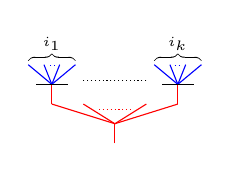
\begin{tikzpicture}[scale=0.2,baseline=(pt_base.base)]

\coordinate (pt_base) at (0,1.25) ;

% étiquettes 

\draw [decorate,    decoration = {calligraphic brace}] (-5.5,4) --  (-2.5,4) ;
\draw [decorate,    decoration = {calligraphic brace}] (2.5,4) --  (5.5,4) ;

\node[above] at (-4,4) {\tiny $i_1$} ; 
\node[above] at (4,4) {\tiny $i_k$} ; 


% arbre inférieur

\draw[red] (-4,1.25) -- (0,0) ;
\draw[red] (-2,1.25) -- (0,0) ;
\draw[red] (4,1.25) -- (0,0) ;
\draw[red] (2,1.25) -- (0,0) ;
\draw[red] (0,-1.25) -- (0,0) ; 

% arbre bicoloré supérieur droit

\draw[blue] (2.5,3.75) -- (4,2.5) ;
\draw[blue] (3.5,3.75) -- (4,2.5) ;
\draw[blue] (4.5,3.75) -- (4,2.5) ;
\draw[blue] (5.5,3.75) -- (4,2.5) ;
\draw[red] (4,1.25) -- (4,2.5) ;

\draw (3,2.5) -- (5,2.5) ;

% arbre bicoloré supérieur droit

\draw[blue] (-2.5,3.75) -- (-4,2.5) ;
\draw[blue] (-3.5,3.75) -- (-4,2.5) ;
\draw[blue] (-4.5,3.75) -- (-4,2.5) ;
\draw[blue] (-5.5,3.75) -- (-4,2.5) ;
\draw[red] (-4,1.25) -- (-4,2.5) ;

\draw (-3,2.5) -- (-5,2.5) ;

% autres traits

\draw [densely dotted,red] (-1,0.9) -- (1,0.9) ;
\draw [densely dotted] (2,2.75) -- (-2,2.75) ; 
\draw [densely dotted,blue] (3.8,3.7) -- (4.2,3.7) ;
\draw [densely dotted,blue] (-3.8,3.7) -- (-4.2,3.7) ;

\end{tikzpicture}}

% Opération unaire de A-infini - Morph

\newcommand{\arbreopunmorph}{
\begin{tikzpicture}[scale=0.15,baseline=(pt_base.base)]

\coordinate (pt_base) at (0,-0.5) ;

\draw[blue] (0,1.25) -- (0,0) ;
\draw[red] (0,-1.25) -- (0,0) ;

\draw (-1.25,0) -- (1.25,0) ;

\end{tikzpicture}
}

\newcommand{\arbreopunmorphcompun}{
\begin{tikzpicture}[scale=0.15,baseline=(pt_base.base)]

\coordinate (pt_base) at (0,-0.5) ;

\draw[blue] (0,1.25) -- (0,0) ;
\draw[orange] (0,-1.25) -- (0,0) ;

\draw (-1.25,0) -- (1.25,0) ;

\end{tikzpicture}
}

\newcommand{\arbreopunmorphcompdeux}{
\begin{tikzpicture}[scale=0.15,baseline=(pt_base.base)]

\coordinate (pt_base) at (0,-0.5) ;

\draw[orange] (0,1.25) -- (0,0) ;
\draw[red] (0,-1.25) -- (0,0) ;

\draw (-1.25,0) -- (1.25,0) ;

\end{tikzpicture}
}

\newcommand{\produitcup}{
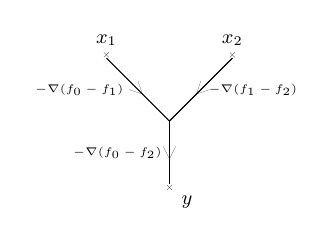
\begin{tikzpicture}[scale=0.8, every node/.style={scale=0.8}]

\draw (-1,1) node[above=2 pt]{\small $x_1$} node[above,scale = 0.08]{\cross} -- (0,0) node{}
node[midway,left = 3 pt]{\tiny $- \nabla (f_0-f_1)$} node[midway,sloped,allow upside down,scale=0.1]{\midarrow} ;
\draw (1,1) node[above=2pt]{\small $x_2$} node[above,scale = 0.08]{\cross} -- (0,0) node{}
node[midway,right]{\tiny $- \nabla (f_1-f_2)$} node[midway,sloped,allow upside down,scale=0.1]{\midarrow} ;
\draw (0,0) node{} -- (0,-1) node[below right  = 2 pt]{\small $y$} node[below ,scale = 0.08]{\cross}
node[midway,left]{\tiny $- \nabla (f_0-f_2)$} node[midway,sloped,allow upside down,scale=0.1]{\midarrow} ;

\end{tikzpicture} }

\newcommand{\arbredegradientexemple}{
\begin{tikzpicture}[scale=0.8, every node/.style={scale=0.8}]

\begin{scope}

\draw (-2,2) node[above=2 pt]{\small $x_1$} node[above,scale = 0.08]{\cross} -- (-1,1) node{}
node[near end,left = 3 pt]{\tiny $- \nabla f$} node[midway,sloped,allow upside down,scale=0.1]{\midarrow} ;
\draw (-1,1) node{} -- (0,0) node{}
node[near end,left = 3 pt]{\tiny $- \nabla f$} node[midway,sloped,allow upside down,scale=0.1]{\midarrow} ;
\draw (2,2) node[above=2pt]{\small $x_3$} node[above,scale = 0.08]{\cross} -- (0,0) node{}
node[near end,right]{\tiny $- \nabla f$} node[midway,sloped,allow upside down,scale=0.1]{\midarrow} ;
\draw (0,0) node{} -- (0,-1) node[below right  = 2 pt]{\small $y$} node[below ,scale = 0.08]{\cross}
node[near end,left]{\tiny $- \nabla f$} node[midway,sloped,allow upside down,scale=0.1]{\midarrow} ;
\draw (0,2) node[above=2 pt]{\small $x_2$} node[above,scale = 0.08]{\cross} -- (-1,1) node{}
node[near end,right]{\tiny $- \nabla f$} node[midway,sloped,allow upside down,scale=0.1]{\midarrow} ;
\end{scope}

\begin{scope}[xshift = 5 cm]
\draw[->=latex] (-3,0) node{} -- (3,0) node{} node[midway,below = 2pt,text width=6 cm, align = center]{\small \noindent Perturbation du champ de gradient négatif au voisinage de chaque sommet de l'arbre} ;
\end{scope}

\begin{scope}[xshift = 10 cm]
\draw (-2,2) node[above=2 pt]{\small $x_1$} node[above,scale = 0.08]{\cross} -- (-1,1) node{}
node[near end,left = 3 pt]{\tiny $- \nabla f$} node[midway,sloped,allow upside down,scale=0.1]{\midarrow} ;
\draw (-1,1) node{} -- (0,0) node{}
node[near end,left = 3 pt]{\tiny $- \nabla f$} node[midway,sloped,allow upside down,scale=0.1]{\midarrow} ;
\draw (2,2) node[above=2pt]{\small $x_3$} node[above,scale = 0.08]{\cross} -- (0,0) node{}
node[near end,right]{\tiny $- \nabla f$} node[midway,sloped,allow upside down,scale=0.1]{\midarrow} ;
\draw (0,0) node{} -- (0,-1) node[below right  = 2 pt]{\small $y$} node[below ,scale = 0.08]{\cross}
node[near end,left]{\tiny $- \nabla f$} node[midway,sloped,allow upside down,scale=0.1]{\midarrow} ;
\draw (0,2) node[above=2 pt]{\small $x_2$} node[above,scale = 0.08]{\cross} -- (-1,1) node{}
node[near end,right]{\tiny $- \nabla f$} node[midway,sloped,allow upside down,scale=0.1]{\midarrow} ;

\node (O) at (0,0) {};
\node (A) at (-1,1) {} ;
\node (a) at ($(A)!0.7!(O)$)  {};
\node (B) at (1,1) {} ;
\node (b) at ($(B)!0.7!(O)$)  {};
\node (C) at (0,-1) {} ;
\node (c) at ($(C)!0.7!(O)$)  {};

\draw [line width = 1.5 pt,red] (a.center) -- (O.center) node[below right,red] {\tiny $ - \nabla f + \mathbb{X}$} ;
\draw [line width = 1.5 pt,red] (b.center) -- (O.center) ;
\draw [line width = 1.5 pt,red] (c.center) -- (O.center) ;

\node (D) at (-2,2) {};
\node (E) at (0,2) {} ;
\node (d) at ($(D)!0.7!(A)$)  {};
\node (e) at ($(E)!0.7!(A)$)  {};
\node (f) at ($(O)!0.7!(A)$)  {};

\draw [line width = 1.5 pt,red] (d.center) -- (A.center) node[below left,red] {\tiny $ - \nabla f + \mathbb{X}$} ;
\draw [line width = 1.5 pt,red] (e.center) -- (A.center) ;
\draw [line width = 1.5 pt,red] (f.center) -- (A.center) ;
\end{scope}

\end{tikzpicture}
}

\newcommand{\trajmorse}{
\begin{tikzpicture}[scale = 0.5, baseline = (pt_base.base)]

\coordinate (pt_base) at (0,-0.2) ;

\node (A) at (-0.25,1) {\small y} ;
\node (B) at (0.25,-1) {\small x} ;
\node[scale = 0.05,yshift = -100 pt] at (A) {\cross} ;
\node[scale = 0.05,yshift = 80 pt] at (B) {\cross} ;

\draw (A) to[out=-90,in=90] (B) node[midway,xshift = -1 pt,rotate = -45,scale=0.1] {\midarrow} ;
\end{tikzpicture}}

\newcommand{\midarrow}{
\begin{tikzpicture}

\draw (-2,1) -- (0,0) ;
\draw (-2,-1) -- (0,0) ;
\end{tikzpicture}}

\newcommand{\cross}{

\begin{tikzpicture}[very thick]
\draw (0.5,0.5) -- (-0.5,-0.5) ;
\draw (-0.5,0.5) -- (0.5,-0.5) ;
\end{tikzpicture}}

\newcommand{\eqainfnmorphun}{
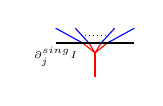
\begin{tikzpicture}[scale=0.25,baseline=(pt_base.base)]

\coordinate (pt_base) at (0,0) ;

\draw (-2,0.5) node[yshift = -5 pt,scale = 0.7]{\tiny $\partial_j^{sing} I$} ;

\draw[blue] (-2,1.25) -- (-0.625,0.5) ;
\draw[blue] (-1,1.25) -- (-0.3125,0.5) ;
\draw[blue] (1,1.25) -- (0.3125,0.5) ;
\draw[blue] (2,1.25) -- (0.625,0.5) ;

\draw[red] (-0.625,0.5) -- (0,0) ;
\draw[red] (-0.3125,0.5) -- (0,0) ;
\draw[red] (0.625,0.5) -- (0,0) ;
\draw[red] (0.3125,0.5) -- (0,0) ;
\draw[red] (0,-1.25) -- (0,0) ;

\draw[blue] [densely dotted] (-0.5,0.9) -- (0.5,0.9) ;

\draw  (-2,0.5) -- (2,0.5) ;

\end{tikzpicture}}

\newcommand{\diagramphilosophy}{
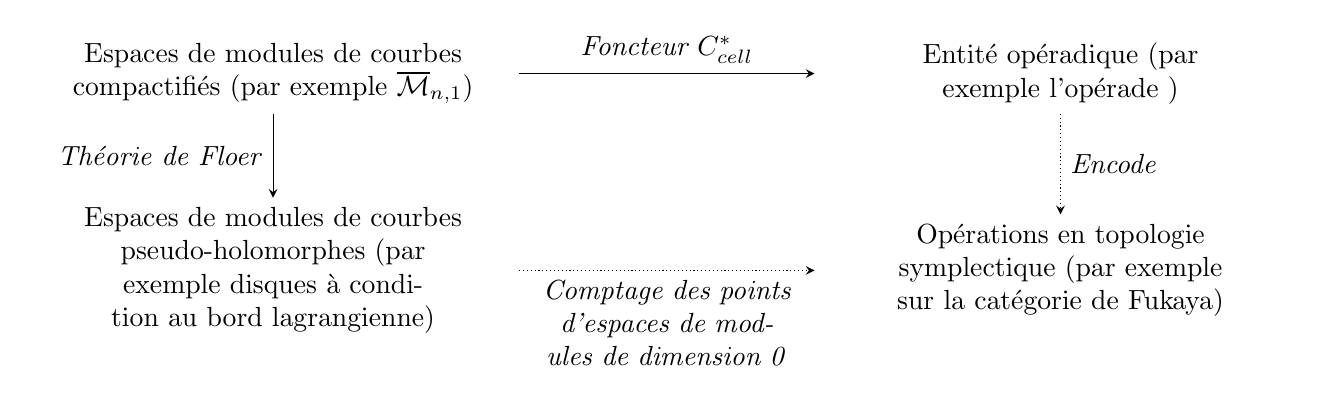
\begin{tikzpicture}[baseline=(pt_base.base)]

\coordinate (pt_base) at (0,-1) ;

\node[text width=6 cm, align = center] (A) at (5,-1) {Opérations en topologie symplectique (par exemple sur la catégorie de Fukaya)} ;
\node[text width=6 cm, align = center] (B) at (-5,-1) {Espaces de modules de courbes pseudo-holomorphes (par exemple disques à condition au bord lagrangienne)} ;
\node[text width=6 cm, align = center] (C) at (-5,1.5) {Espaces de modules de courbes compactifiés (par exemple $\overline{\mathcal{M}}_{n,1}$)} ;
\node[text width=6 cm, align = center] (D) at (5,1.5) {Entité opéradique (par exemple l'opérade \Ainf )} ;

\draw[->,>=stealth,densely dotted] (D) -- (A) node[midway,right] {\Small \textit{Encode}} ;
\draw[->,>=stealth,densely dotted] (B) -- (A) node[midway,below,text width=4.5 cm, align = center] {\Small \textit{Comptage des points d'espaces de modules de dimension 0}} ;
\draw[->,>=stealth] (C) -- (B) node[midway,left] {\Small \textit{Théorie de Floer}} ;
\draw[->,>=stealth] (C) -- (D) node[midway,above] {\Small \textit{Foncteur $C^*_{cell}$}} ;
\end{tikzpicture}
}

\newcommand{\eqainfnmorphdeux}{
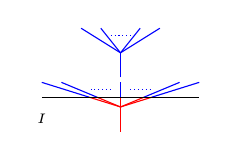
\begin{tikzpicture}[scale=0.25,baseline=(pt_base.base)]

\coordinate (pt_base) at (0,1.25) ;

% traits bicolorés

\draw[blue] (-4,1.25) -- (-1.6,0.5) ;
\draw[blue] (-3,1.25) -- (-1.2,0.5) ;
\draw[blue] (4,1.25) -- (1.6,0.5) ;
\draw[blue] (3,1.25) -- (1.2,0.5) ;
\draw[blue] (0,1.25) -- (0,0.5) ;

\draw[red] (-1.6,0.5) -- (0,0) ;
\draw[red] (-1.2,0.5) -- (0,0) ;
\draw[red] (1.6,0.5) -- (0,0) ;
\draw[red] (1.2,0.5) -- (0,0) ;
\draw[red] (0,0.5) -- (0,0) ;
\draw[red] (0,-1.25) -- (0,0) ; 

% traits arbre supérieur

\draw[blue] (-2,4) -- (0,2.75) ;
\draw[blue] (-1,4) -- (0,2.75) ;
\draw[blue] (1,4) -- (0,2.75) ;
\draw[blue] (2,4) -- (0,2.75) ;
\draw[blue] (0,1.5) -- (0,2.75) ;

% autres traits

\draw[blue] [densely dotted] (-0.5,3.65) -- (0.5,3.65) ;
\draw[blue] [densely dotted] (-0.5,0.9) -- (-1.5,0.9) ;
\draw[blue] [densely dotted] (0.5,0.9) -- (1.5,0.9) ;

\draw (-4,0.5) -- (4,0.5) ;

\draw (-4,0.5) node[yshift = - 8 pt] {\tiny $I$} ;

\end{tikzpicture}}

\newcommand{\eqainf}{
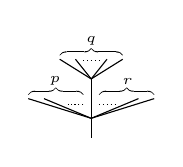
\begin{tikzpicture}[scale=0.2,baseline=(pt_base.base)]

\coordinate (pt_base) at (0,1.25) ;

\draw [decorate,    decoration = {calligraphic brace}] (-4,1.5) --  (-0.5,1.5) ;
\draw [decorate,    decoration = {calligraphic brace}] (0.5,1.5) --  (4,1.5) ;
\draw [decorate,    decoration = {calligraphic brace}] (-2,4) --  (2,4) ;

\node[above] at (-2.3,1.5) {\tiny $p$} ; 
\node[above] at (0,4) {\tiny $q$} ; 
\node[above] at (2.3,1.5) {\tiny $r$} ; 

\draw (-4,1.25) -- (0,0) ;
\draw (-3,1.25) -- (0,0) ;
\draw (4,1.25) -- (0,0) ;
\draw (3,1.25) -- (0,0) ;
\draw (0,1.25) -- (0,0) ;
\draw(0,-1.25) -- (0,0) ; 

\draw (-2,3.75) -- (0,2.5) ;
\draw (-1,3.75) -- (0,2.5) ;
\draw (1,3.75) -- (0,2.5) ;
\draw (2,3.75) -- (0,2.5) ;
\draw (0,1.25) -- (0,2.5) ;

\draw [densely dotted] (-0.5,3.65) -- (0.5,3.65) ;
\draw [densely dotted] (-0.5,0.9) -- (-1.5,0.9) ;
\draw [densely dotted] (0.5,0.9) -- (1.5,0.9) ;

\end{tikzpicture}}

\newcommand{\eqainfnmorphtrois}{
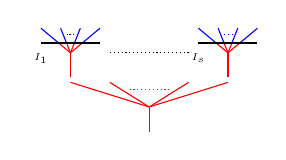
\begin{tikzpicture}[scale=0.25,baseline=(pt_base.base)]

\coordinate (pt_base) at (0,1.25) ;

% arbre inférieur

\draw[red] (-4,1.25) -- (0,0) ;
\draw[red] (-2,1.25) -- (0,0) ;
\draw[red] (4,1.25) -- (0,0) ;
\draw[red] (2,1.25) -- (0,0) ;
\draw[red] (0,-1.25) -- (0,0) ; 

% arbre bicoloré supérieur droit

\draw[blue] (2.5,4) -- (3.4,3.25) ;
\draw[blue] (3.5,4) -- (3.8,3.25) ;
\draw[blue] (4.5,4) -- (4.2,3.25) ;
\draw[blue] (5.5,4) -- (4.6,3.25) ;

\draw[red] (3.4,3.25) -- (4,2.75) ;
\draw[red] (3.8,3.25) -- (4,2.75) ;
\draw[red] (4.2,3.25) -- (4,2.75) ;
\draw[red] (4.6,3.25) -- (4,2.75) ;
\draw[red] (4,1.5) -- (4,2.75) ;

\draw (2.5,3.25) -- (5.5,3.25) ;

\draw (2.5,3.25) node[scale = 0.7,yshift = - 8 pt] {\tiny $I_s$} ;

% arbre bicoloré supérieur droit

\draw[blue] (-2.5,4) -- (-3.4,3.25) ;
\draw[blue] (-3.5,4) -- (-3.8,3.25) ;
\draw[blue] (-4.5,4) -- (-4.2,3.25) ;
\draw[blue] (-5.5,4) -- (-4.6,3.25) ;

\draw[red] (-3.4,3.25) -- (-4,2.75) ;
\draw[red] (-3.8,3.25) -- (-4,2.75) ;
\draw[red] (-4.2,3.25) -- (-4,2.75) ;
\draw[red] (-4.6,3.25) -- (-4,2.75) ;
\draw[red] (-4,1.5) -- (-4,2.75) ;

\draw (-2.5,3.25) -- (-5.5,3.25) ;

\draw (-5.5,3.25) node[scale = 0.7,yshift = - 8 pt] {\tiny $I_1$} ;

% autres traits

\draw [densely dotted,red] (-1,0.9) -- (1,0.9) ;
\draw [densely dotted] (2,2.75) -- (-2,2.75) ; 
\draw [densely dotted,blue] (3.8,3.7) -- (4.2,3.7) ;
\draw [densely dotted,blue] (-3.8,3.7) -- (-4.2,3.7) ;

\end{tikzpicture}}

\newcommand{\eqainfnmorphquatre}{
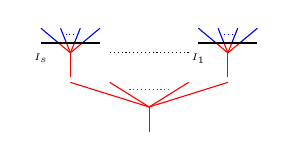
\begin{tikzpicture}[scale=0.25,baseline=(pt_base.base)]

\coordinate (pt_base) at (0,1.25) ;

% arbre inférieur

\draw[red] (-4,1.25) -- (0,0) ;
\draw[red] (-2,1.25) -- (0,0) ;
\draw[red] (4,1.25) -- (0,0) ;
\draw[red] (2,1.25) -- (0,0) ;
\draw[red] (0,-1.25) -- (0,0) ; 

% arbre bicoloré supérieur droit

\draw[blue] (2.5,4) -- (3.4,3.25) ;
\draw[blue] (3.5,4) -- (3.8,3.25) ;
\draw[blue] (4.5,4) -- (4.2,3.25) ;
\draw[blue] (5.5,4) -- (4.6,3.25) ;

\draw[red] (3.4,3.25) -- (4,2.75) ;
\draw[red] (3.8,3.25) -- (4,2.75) ;
\draw[red] (4.2,3.25) -- (4,2.75) ;
\draw[red] (4.6,3.25) -- (4,2.75) ;
\draw[red] (4,1.5) -- (4,2.75) ;

\draw (2.5,3.25) -- (5.5,3.25) ;

\draw (2.5,3.25) node[scale = 0.7,yshift = - 8 pt] {\tiny $I_1$} ;
% arbre bicoloré supérieur droit

\draw[blue] (-2.5,4) -- (-3.4,3.25) ;
\draw[blue] (-3.5,4) -- (-3.8,3.25) ;
\draw[blue] (-4.5,4) -- (-4.2,3.25) ;
\draw[blue] (-5.5,4) -- (-4.6,3.25) ;

\draw[red] (-3.4,3.25) -- (-4,2.75) ;
\draw[red] (-3.8,3.25) -- (-4,2.75) ;
\draw[red] (-4.2,3.25) -- (-4,2.75) ;
\draw[red] (-4.6,3.25) -- (-4,2.75) ;
\draw[red] (-4,1.5) -- (-4,2.75) ;

\draw (-2.5,3.25) -- (-5.5,3.25) ;

\draw (-5.5,3.25) node[scale = 0.7,yshift = - 8 pt] {\tiny $I_s$} ;

% autres traits

\draw [densely dotted,red] (-1,0.9) -- (1,0.9) ;
\draw [densely dotted] (2,2.75) -- (-2,2.75) ; 
\draw [densely dotted,blue] (3.8,3.7) -- (4.2,3.7) ;
\draw [densely dotted,blue] (-3.8,3.7) -- (-4.2,3.7) ;

\end{tikzpicture}}

% Associaèdre de dimension 3

\newcommand{\arbreoptdAB}{
\begin{tikzpicture}
\begin{scope}
\draw (0,1.25) -- (0,0) ;
\draw (-1.25,1.25) -- (0,0) ;
\draw (1.25,1.25) -- (0,0) ;
\draw (0,-1.25) -- (0,0) ;
\end{scope}

\begin{scope}[shift = {(1.25,3)}]
\draw (-1.25,1.25) -- (0,0) ;
\draw (1.25,1.25) -- (0,0) ;
\draw (0,-1.25) -- (0,0) ;
\end{scope}
\end{tikzpicture}
}

\newcommand{\arbreoptdDE}{
\begin{tikzpicture}
\begin{scope}
\draw (0,1.25) -- (0,0) ;
\draw (-1.25,1.25) -- (0,0) ;
\draw (1.25,1.25) -- (0,0) ;
\draw (0,-1.25) -- (0,0) ;
\end{scope}

\begin{scope}[shift = {(0,3)}]
\draw (-1.25,1.25) -- (0,0) ;
\draw (1.25,1.25) -- (0,0) ;
\draw (0,-1.25) -- (0,0) ;
\end{scope}
\end{tikzpicture}
}

\newcommand{\arbreoptdBC}{
\begin{tikzpicture}
\begin{scope}
\draw (0,1.25) -- (0,0) ;
\draw (-1.25,1.25) -- (0,0) ;
\draw (1.25,1.25) -- (0,0) ;
\draw (0,-1.25) -- (0,0) ;
\end{scope}

\begin{scope}[shift = {(-1.25,3)}]
\draw (-1.25,1.25) -- (0,0) ;
\draw (1.25,1.25) -- (0,0) ;
\draw (0,-1.25) -- (0,0) ;
\end{scope}
\end{tikzpicture}
}

\newcommand{\arbreoptdEA}{
\begin{tikzpicture}

\begin{scope}
\draw (-1.25,1.25) -- (0,0) ;
\draw (1.25,1.25) -- (0,0) ;
\draw (0,-1.25) -- (0,0) ;
\end{scope}

\begin{scope}[shift = {(1.25,3)}]
\draw (0,1.25) -- (0,0) ;
\draw (-1.25,1.25) -- (0,0) ;
\draw (1.25,1.25) -- (0,0) ;
\draw (0,-1.25) -- (0,0) ;
\end{scope}

\end{tikzpicture}
}

\newcommand{\arbreoptdCD}{
\begin{tikzpicture}
\begin{scope}
\draw (-1.25,1.25) -- (0,0) ;
\draw (1.25,1.25) -- (0,0) ;
\draw (0,-1.25) -- (0,0) ;
\end{scope}

\begin{scope}[shift = {(-1.25,3)}]
\draw (0,1.25) -- (0,0) ;
\draw (-1.25,1.25) -- (0,0) ;
\draw (1.25,1.25) -- (0,0) ;
\draw (0,-1.25) -- (0,0) ;
\end{scope}
\end{tikzpicture}
}

\newcommand{\arbreopdddC}{
\begin{tikzpicture}

\begin{scope}
\draw (-1.25,1.25) -- (0,0) ;
\draw (1.25,1.25) -- (0,0) ;
\draw (0,-1.25) -- (0,0) ;
\end{scope}

\begin{scope}[shift = {(-1.25,3)}]
\draw (-1.25,1.25) -- (0,0) ;
\draw (1.25,1.25) -- (0,0) ;
\draw (0,-1.25) -- (0,0) ;
\end{scope}

\begin{scope}[shift = {(-2.5,6)}]
\draw (-1.25,1.25) -- (0,0) ;
\draw (1.25,1.25) -- (0,0) ;
\draw (0,-1.25) -- (0,0) ;
\end{scope}
\end{tikzpicture}
}

\newcommand{\arbreopdddB}{
\begin{tikzpicture}

\begin{scope}
\draw (-1.25,1.25) -- (0,0) ;
\draw (1.25,1.25) -- (0,0) ;
\draw (0,-1.25) -- (0,0) ;
\end{scope}

\begin{scope}[shift = {(-1.4,3)}]
\draw (-1.25,1.25) -- (0,0) ;
\draw (1.25,1.25) -- (0,0) ;
\draw (0,-1.25) -- (0,0) ;
\end{scope}

\begin{scope}[shift = {(1.4,3)}]
\draw (-1.25,1.25) -- (0,0) ;
\draw (1.25,1.25) -- (0,0) ;
\draw (0,-1.25) -- (0,0) ;
\end{scope}
\end{tikzpicture}
}

\newcommand{\arbreopdddA}{
\begin{tikzpicture}

\begin{scope}
\draw (-1.25,1.25) -- (0,0) ;
\draw (1.25,1.25) -- (0,0) ;
\draw (0,-1.25) -- (0,0) ;
\end{scope}

\begin{scope}[shift = {(1.25,3)}]
\draw (-1.25,1.25) -- (0,0) ;
\draw (1.25,1.25) -- (0,0) ;
\draw (0,-1.25) -- (0,0) ;
\end{scope}

\begin{scope}[shift = {(2.5,6)}]
\draw (-1.25,1.25) -- (0,0) ;
\draw (1.25,1.25) -- (0,0) ;
\draw (0,-1.25) -- (0,0) ;
\end{scope}
\end{tikzpicture}
}

\newcommand{\arbreopdddE}{
\begin{tikzpicture}

\begin{scope}
\draw (-1.25,1.25) -- (0,0) ;
\draw (1.25,1.25) -- (0,0) ;
\draw (0,-1.25) -- (0,0) ;
\end{scope}

\begin{scope}[shift = {(1.25,3)}]
\draw (-1.25,1.25) -- (0,0) ;
\draw (1.25,1.25) -- (0,0) ;
\draw (0,-1.25) -- (0,0) ;
\end{scope}

\begin{scope}[shift = {(0,6)}]
\draw (-1.25,1.25) -- (0,0) ;
\draw (1.25,1.25) -- (0,0) ;
\draw (0,-1.25) -- (0,0) ;
\end{scope}
\end{tikzpicture}
}


\newcommand{\arbreopdddD}{
\begin{tikzpicture}

\begin{scope}
\draw (-1.25,1.25) -- (0,0) ;
\draw (1.25,1.25) -- (0,0) ;
\draw (0,-1.25) -- (0,0) ;
\end{scope}

\begin{scope}[shift = {(-1.25,3)}]
\draw (-1.25,1.25) -- (0,0) ;
\draw (1.25,1.25) -- (0,0) ;
\draw (0,-1.25) -- (0,0) ;
\end{scope}

\begin{scope}[shift = {(0,6)}]
\draw (-1.25,1.25) -- (0,0) ;
\draw (1.25,1.25) -- (0,0) ;
\draw (0,-1.25) -- (0,0) ;
\end{scope}
\end{tikzpicture}
}

% Associaèdre subdivisé 

\newcommand{\TquatrestratCbis}{
\begin{tikzpicture}
\node (A) at (0,0) {} ;
\node (B) at (0,-1) {} ;
\node (C) at (-2,2) {} ;
\node (D) at (-1,1) {} ;
\node (E) at (0,2) {} ;
\node (F) at (-1.5,1.5) {} ;
\node (G) at (-1,2) {} ;
\node (H) at (2,2) {} ;

\draw (C.center) -- (F.center) -- (D.center) -- (A.center) -- (B.center) ;
\draw (A.center) -- (H.center) ;
\draw (D.center) -- (E.center) ;
\draw (F.center) -- (G.center) ;
\end{tikzpicture}
}

\newcommand{\TquatrestratAbis}{
\begin{tikzpicture}
\node (A) at (0,0) {} ;
\node (B) at (0,-1) {} ;
\node (C) at (-2,2) {} ;
\node (D) at (1,1) {} ;
\node (E) at (0,2) {} ;
\node (F) at (1.5,1.5) {} ;
\node (G) at (1,2) {} ;
\node (H) at (2,2) {} ;

\draw (H.center) -- (F.center) -- (D.center) -- (A.center) -- (B.center) ;
\draw (A.center) -- (C.center) ;
\draw (D.center) -- (E.center) ;
\draw (F.center) -- (G.center) ;
\end{tikzpicture}
}

\newcommand{\TquatrestratBbis}{
\begin{tikzpicture}
\node (A) at (-1.5,1) {} ;
\node (B) at (0,0) {} ;
\node (C) at (1.5,1) {} ;
\node (D) at (0,-1) {} ;
\node (E) at (0.25,2) {} ;
\node (F) at (2.75,2) {} ;
\node (G) at (-0.25,2) {} ;
\node (I) at (-2.75,2) {} ;

\draw (I.center) -- (A.center) -- (B.center) -- (C.center) -- (E.center) ;
\draw (F.center) -- (C.center) ;
\draw (G.center) -- (A.center) ;
\draw (B.center) -- (D.center) ;
\end{tikzpicture}
}

\newcommand{\TquatrestratEbis}{
\begin{tikzpicture}
\node (A) at (0,0) {} ;
\node (B) at (2,2) {} ;
\node (H) at (-2,2) {} ;
\node (C) at (0,2) {} ;
\node (E) at (0.5,1.5) {} ;
\node (F) at (1,2) {} ;
\node (G) at (0,-1) {} ;
\node (D) at (1,1) {} ;

\draw (C.center) -- (E.center) -- (D.center) -- (A.center) -- (G.center) ;
\draw (A.center) -- (H.center) ;
\draw (E.center) -- (F.center) ;
\draw (B.center) -- (D.center) ;
\end{tikzpicture}
}

\newcommand{\TquatrestratDbis}{
\begin{tikzpicture}
\node (A) at (0,0) {} ;
\node (B) at (0,-1) {} ;
\node (C) at (-2,2) {} ;
\node (D) at (-1,1) {} ;
\node (E) at (0,2) {} ;
\node (F) at (-0.5,1.5) {} ;
\node (G) at (-1,2) {} ;
\node (H) at (2,2) {} ;

\draw (E.center) -- (F.center) -- (D.center) -- (A.center) -- (B.center) ;
\draw (A.center) -- (H.center) ;
\draw (G.center) -- (F.center) ;
\draw (C.center) -- (D.center) ;
\end{tikzpicture}
}

\newcommand{\Tquatrestratbis}{
\begin{tikzpicture}[scale = 0.6, baseline = (pt_base.base)]

\coordinate (pt_base) at (-1,0) ; 

\node[scale = 0.2] (Ap) at (0.6,1.6) {\TquatrestratAbis} ;
\node[scale = 0.2] (Bp) at (-0.7,-0.2) {\TquatrestratBbis} ;
\node[scale = 0.2] (Cp) at (0.5,-1.7) {\TquatrestratCbis} ;
\node[scale = 0.2] (Dp) at (2.7,-0.9) {\TquatrestratDbis} ;
\node[scale = 0.2] (Ep) at (2.8,0.9) {\TquatrestratEbis} ;

\node[scale = 0.1] (A) at (0,3) {} ;
\node[scale = 0.1] (B) at (-2,0) {} ;
\node[scale = 0.1] (C) at (0,-3) {} ;
\node[scale = 0.1] (D) at (4,-1.5) {} ;
\node[scale = 0.1] (E) at (4,1.5) {} ;
\node (O) at (1,0) {} ;

\draw[fill,opacity = 0.1] (A.center) -- (B.center) -- (C.center) -- (D.center) -- (E.center) -- (A.center) ;

\draw (A.center) -- (B.center) -- (C.center) -- (D.center) -- (E.center) -- (A.center) ;

\draw ($(A)!0.5!(B)$) -- (O.center) ;
\draw ($(B)!0.5!(C)$) -- (O.center) ;
\draw ($(C)!0.5!(D)$) -- (O.center) ;
\draw ($(D)!0.5!(E)$) -- (O.center) ;
\draw ($(E)!0.5!(A)$) -- (O.center) ;

\node[scale=0.1] at (A) {\pointbullet} ;
\node[scale=0.1] at (B) {\pointbullet} ;
\node[scale=0.1] at (C) {\pointbullet} ;
\node[scale=0.1] at (D) {\pointbullet} ;
\node[scale=0.1] at (E) {\pointbullet} ;



\end{tikzpicture}}

\newcommand{\associaedretrois}{
\begin{tikzpicture}[scale = 0.5 , baseline = (pt_base.base)]

\coordinate (pt_base) at (-1,0) ; 

\node[scale = 0.1] (A) at (0,3) {} ;
\node[scale=0.1,above = 5pt] at (A) {\arbreopdddA} ;
\node[scale = 0.1] (B) at (-2,0) {} ;
\node[scale = 0.1,left = 5 pt] at (B) {\arbreopdddB} ;
\node[scale = 0.1] (C) at (0,-3) {} ;
\node[scale = 0.1 , below left = 5 pt] at (C) {\arbreopdddC} ;
\node[scale = 0.1] (D) at (4,-1.5) {} ;
\node[scale = 0.1,below right = 7 pt] at (D) {\arbreopdddD} ;
\node[scale = 0.1] (E) at (4,1.5) {} ;
\node[scale = 0.1,above right = 7 pt] at (E) {\arbreopdddE} ;

\node at (1,0) {\arbreopquatre} ;

\draw[fill,opacity = 0.1] (A.center) -- (B.center) -- (C.center) -- (D.center) -- (E.center) -- (A.center) ;

\draw (A.center) -- (B.center) -- (C.center) -- (D.center) -- (E.center) -- (A.center) ;

\node[scale=0.1] at (A) {\pointbullet} ;
\node[scale=0.1] at (B) {\pointbullet} ;
\node[scale=0.1] at (C) {\pointbullet} ;
\node[scale=0.1] at (D) {\pointbullet} ;
\node[scale=0.1] at (E) {\pointbullet} ;

\node[scale = 0.1,above left = 3 pt] at ($(A)!0.5!(B)$) {\arbreoptdAB} ;
\node[scale = 0.1,below left = 3 pt] at ($(B)!0.5!(C)$) {\arbreoptdBC} ;
\node[scale = 0.1,below right = 6 pt] at ($(C)!0.5!(D)$) {\arbreoptdCD} ;
\node[scale = 0.1,right = 2 pt] at ($(D)!0.5!(E)$) {\arbreoptdDE} ;
\node[scale = 0.1,above right = 6 pt] at ($(E)!0.5!(A)$) {\arbreoptdEA} ;

\end{tikzpicture}
}

\newcommand{\CTtroisstratAbis}{
\begin{tikzpicture}
\node (A) at (0,0) {} ;
\node (B) at (0,-1) {} ;
\node (C) at (1.25,1.25) {} ;
\node (D) at (-1.25,1.25) {} ;
\node (E) at (0,1.25) {} ;
\node (F) at (0.625,0.625) {} ;
\node (G) at (0,-0.3) {} ;
\node (H) at (-1.25,-0.3) {} ;
\node (I) at (1.25,-0.3) {}  ;
\node (J) at (1.5,-0.3) {} ;
\node (K) at (1.5,0) {} ;

\draw[blue] (D.center) -- (A.center) ;
\draw[blue] (A.center) -- (G.center) ;
\draw[blue] (A.center) -- (F.center) ;
\draw[blue] (F.center) -- (E.center) ;
\draw[blue] (C.center) -- (F.center) ;

\draw[red] (G.center) -- (B.center) ;

\draw (H.center) -- (I.center) ;

\end{tikzpicture}}

\newcommand{\CTtroisstratBbis}{
\begin{tikzpicture}
\node (A) at (0,0) {} ;
\node (B) at (0,-1) {} ;
\node (C) at (1.25,1.25) {} ;
\node (D) at (-1.25,1.25) {} ;
\node (E) at (0,1.25) {} ;
\node (F) at (0.625,0.625) {} ;
\node (G) at (-1.25,0.3) {} ;
\node (H) at (1.25,0.3) {} ;
\node (I) at (1.5,0.3) {}  ;
\node (J) at (1.5,0) {} ;

\node (K) at (-0.3,0.3) {} ;
\node (L) at (0.3,0.3) {} ;

\draw[blue] (D.center) -- (K.center) ;
\draw[blue] (L.center) -- (F.center) ;
\draw[blue] (F.center) -- (E.center) ;
\draw[blue] (F.center) -- (C.center) ;
\draw[red] (K.center) -- (A.center) ;
\draw[red] (L.center) -- (A.center) ;
\draw[red] (A.center) -- (B.center) ;
\draw (G.center) -- (H.center) ;
\end{tikzpicture}}

\newcommand{\CTtroisstratCbis}{
\begin{tikzpicture}
\node (A) at (0,0) {} ;
\node (B) at (0,-1) {} ;
\node (C) at (1.25,1.25) {} ;
\node (D) at (-1.25,1.25) {} ;
\node (E) at (0,1.25) {} ;
\node (F) at (0.625,0.625) {} ;
\node (G) at (-0.9,0.9) {} ;
\node (H) at (0.35,0.9) {} ;
\node (I) at (0.9,0.9) {}  ;
\node (J) at (-1.25,0.9) {} ;
\node (K) at (1.25,0.9) {} ;
\node (L) at (1.5,0) {} ;
\node (M) at (1.5,0.9) {} ;

\draw[blue] (D.center) -- (G.center) ;
\draw[blue] (E.center) -- (H.center) ;
\draw[blue] (C.center) -- (I.center) ;

\draw[red] (G.center) -- (A.center) ;
\draw[red] (H.center) -- (F.center) ;
\draw[red] (F.center) -- (A.center) ;
\draw[red] (A.center) -- (I.center) ;
\draw[red] (A.center) -- (B.center) ;

\draw (J.center) -- (K.center) ;

\end{tikzpicture}}

\newcommand{\CTtroisstratDbis}{
\begin{tikzpicture}
\node (A) at (0,0) {} ;
\node (B) at (0,-1) {} ;
\node (C) at (1.25,1.25) {} ;
\node (D) at (-1.25,1.25) {} ;
\node (E) at (0,1.25) {} ;
\node (F) at (-0.625,0.625) {} ;
\node (G) at (-0.9,0.9) {} ;
\node (H) at (-0.35,0.9) {} ;
\node (I) at (0.9,0.9) {}  ;
\node (J) at (-1.25,0.9) {} ;
\node (K) at (1.25,0.9) {} ;
\node (L) at (1.5,0) {} ;
\node (M) at (1.5,0.9) {} ;

\draw[blue] (D.center) -- (G.center) ;
\draw[blue] (E.center) -- (H.center) ;
\draw[blue] (C.center) -- (I.center) ;

\draw[red] (G.center) -- (F.center) ;
\draw[red] (H.center) -- (F.center) ;
\draw[red] (F.center) -- (A.center) ;
\draw[red] (A.center) -- (I.center) ;
\draw[red] (A.center) -- (B.center) ;

\draw (J.center) -- (K.center) ;

\end{tikzpicture}}

\newcommand{\CTtroisstratEbis}{
\begin{tikzpicture}
\node (A) at (0,0) {} ;
\node (B) at (0,-1) {} ;
\node (C) at (1.25,1.25) {} ;
\node (D) at (-1.25,1.25) {} ;
\node (E) at (0,1.25) {} ;
\node (F) at (-0.625,0.625) {} ;
\node (G) at (-1.25,0.3) {} ;
\node (H) at (1.25,0.3) {} ;
\node (I) at (1.5,0.3) {}  ;
\node (J) at (1.5,0) {} ;

\node (K) at (-0.3,0.3) {} ;
\node (L) at (0.3,0.3) {} ;

\draw[blue] (D.center) -- (F.center) -- (K.center) ;
\draw[red] (K.center) -- (A.center) ;
\draw[blue] (F.center) -- (E.center) ;
\draw[red] (A.center) -- (B.center) ;
\draw[red] (A.center) -- (L.center) ;
\draw[blue] (L.center) -- (C.center) ;
\draw[blue] (F.center) -- (E.center) ;
\draw (G.center) -- (H.center) ;
\end{tikzpicture}}

\newcommand{\CTtroisstratFbis}{
\begin{tikzpicture}
\node (A) at (0,0) {} ;
\node (B) at (0,-1) {} ;
\node (C) at (1.25,1.25) {} ;
\node (D) at (-1.25,1.25) {} ;
\node (E) at (0,1.25) {} ;
\node (F) at (-0.625,0.625) {} ;
\node (G) at (0,-0.3) {} ;
\node (H) at (-1.25,-0.3) {} ;
\node (I) at (1.25,-0.3) {}  ;
\node (J) at (1.5,-0.3) {} ;
\node (K) at (1.5,0) {} ;

\draw[blue] (D.center) -- (A.center) ;
\draw[blue] (A.center) -- (G.center) ;
\draw[blue] (A.center) -- (F.center) ;
\draw[blue] (F.center) -- (E.center) ;
\draw[blue] (C.center) -- (A.center) ;

\draw[red] (G.center) -- (B.center) ;

\draw (H.center) -- (I.center) ;

\end{tikzpicture}}

\newcommand{\CTtroisstratbis}{
\begin{tikzpicture}[scale = 1.3 , baseline = (pt_base.base)]

\coordinate (pt_base) at (-1,0) ;

\node[scale = 0.34] (Ap) at (0.52,-0.82) {\CTtroisstratAbis} ;
\node[scale = 0.34] (Bp) at (1.1,0) {\CTtroisstratBbis} ;
\node[scale = 0.34] (Cp) at (0.5,0.8) {\CTtroisstratCbis} ;
\node[scale = 0.34] (Dp) at (-0.4,0.8) {\CTtroisstratDbis} ;
\node[scale = 0.34] (Ep) at (-0.9,0) {\CTtroisstratEbis} ; 
\node[scale = 0.34] (Fp) at (-0.4,-0.8) {\CTtroisstratFbis} ; 

\node[scale = 0.1] (A) at (0.85,-1.4) {} ;
\node[scale = 0.1] (B) at (1.65,0) {} ;
\node[scale = 0.1] (C) at (0.85,1.35) {} ;
\node[scale = 0.1] (D) at (-0.75,1.35) {} ;
\node[scale = 0.1] (E) at (-1.5,0) {} ;
\node[scale = 0.1] (F) at (-0.75,-1.4) {} ;

\node (O) at (0,0) {} ;

\draw[fill,opacity = 0.1] (A.center) -- (B.center) -- (C.center) -- (D.center) -- (E.center) -- (F.center) -- (A.center) ;

\draw (A.center) -- (B.center) -- (C.center) -- (D.center) -- (E.center) -- (F.center) -- (A.center) ;

\node[scale=0.1] at (A) {\pointbullet} ;
\node[scale=0.1] at (B) {\pointbullet} ;
\node[scale=0.1] at (C) {\pointbullet} ;
\node[scale=0.1] at (D) {\pointbullet} ;
\node[scale=0.1] at (E) {\pointbullet} ;
\node[scale=0.1] at (F) {\pointbullet} ;

\draw ($(A)!0.5!(B)$) --(O.center) ;
\draw ($(B)!0.5!(C)$) --(O.center) ;
\draw ($(C)!0.5!(D)$) --(O.center) ;
\draw ($(D)!0.5!(E)$) --(O.center) ;
\draw ($(E)!0.5!(F)$) --(O.center) ;
\draw ($(F)!0.5!(A)$) --(O.center) ;
\end{tikzpicture}
}

%multiplaèdre

\newcommand{\multiplaedretroisA}{
\begin{tikzpicture}

\begin{scope}
\draw[blue] (0,1.25) -- (0,0.5) ;
\draw[red] (0,-1.25) -- (0,0.5) ;

\draw (-1.25,0.5) -- (1.25,0.5) ;
\end{scope}

\begin{scope}[shift = {(0,3)},blue]
\draw (-1.25,1.25) -- (0,0) ;
\draw (1.25,1.25) -- (0,0) ;
\draw (0,-1.25) -- (0,0) ;
\end{scope}

\begin{scope}[shift = {(1.25,6)},blue]
\draw (-1.25,1.25) -- (0,0) ;
\draw (1.25,1.25) -- (0,0) ;
\draw (0,-1.25) -- (0,0) ;
\end{scope}
\end{tikzpicture}
}

\newcommand{\multiplaedretroisB}{
\begin{tikzpicture}


\begin{scope}[red]
\draw (-1.25,1.25) -- (0,0) ;
\draw (1.25,1.25) -- (0,0) ;
\draw (0,-1.25) -- (0,0) ;
\end{scope}

\begin{scope}[shift = {(-1.25,3)}]
\draw[blue] (0,1.25) -- (0,0.5) ;
\draw[red] (0,-1.25) -- (0,0.5) ;

\draw (-1.25,0.5) -- (0.75,0.5) ;
\end{scope}

\begin{scope}[shift = {(1.25,3)}]
\draw[blue] (0,1.25) -- (0,0.5) ;
\draw[red] (0,-1.25) -- (0,0.5) ;

\draw (-0.75,0.5) -- (1.25,0.5) ;
\end{scope}

\begin{scope}[shift = {(1.25,6)},blue]
\draw (-1.25,1.25) -- (0,0) ;
\draw (1.25,1.25) -- (0,0) ;
\draw (0,-1.25) -- (0,0) ;
\end{scope}
\end{tikzpicture}
}

\newcommand{\multiplaedretroisC}{
\begin{tikzpicture}

\begin{scope}[red]
\draw (-1.25,1.25) -- (0,0) ;
\draw (1.25,1.25) -- (0,0) ;
\draw (0,-1.25) -- (0,0) ;
\end{scope}

\begin{scope}[shift = {(1.25,3)},red]
\draw (-1.25,1.25) -- (0,0) ;
\draw (1.25,1.25) -- (0,0) ;
\draw (0,-1.25) -- (0,0) ;
\end{scope}

\begin{scope}[shift = {(2.5,6)}]
\draw[blue] (0,1.25) -- (0,0.5) ;
\draw[red] (0,-1.25) -- (0,0.5) ;

\draw (-0.75,0.5) -- (1.25,0.5) ;
\end{scope}

\begin{scope}[shift = {(0,6)}]
\draw[blue] (0,1.25) -- (0,0.5) ;
\draw[red] (0,-1.25) -- (0,0.5) ;

\draw (-1.25,0.5) -- (0.75,0.5) ;
\end{scope}

\begin{scope}[shift = {(-1.25,3)}]
\draw[blue] (0,1.25) -- (0,0.5) ;
\draw[red] (0,-1.25) -- (0,0.5) ;

\draw (-1.25,0.5) -- (1.25,0.5) ;
\end{scope}

\end{tikzpicture}
}

\newcommand{\multiplaedretroisD}{
\begin{tikzpicture}

\begin{scope}[red]
\draw (-1.25,1.25) -- (0,0) ;
\draw (1.25,1.25) -- (0,0) ;
\draw (0,-1.25) -- (0,0) ;
\end{scope}

\begin{scope}[shift = {(-1.25,3)},red]
\draw (-1.25,1.25) -- (0,0) ;
\draw (1.25,1.25) -- (0,0) ;
\draw (0,-1.25) -- (0,0) ;
\end{scope}

\begin{scope}[shift = {(-2.5,6)}]
\draw[blue] (0,1.25) -- (0,0.5) ;
\draw[red] (0,-1.25) -- (0,0.5) ;

\draw (-1.25,0.5) -- (0.75,0.5) ;
\end{scope}

\begin{scope}[shift = {(0,6)}]
\draw[blue] (0,1.25) -- (0,0.5) ;
\draw[red] (0,-1.25) -- (0,0.5) ;

\draw (-0.75,0.5) -- (1.25,0.5) ;
\end{scope}

\begin{scope}[shift = {(1.25,3)}]
\draw[blue] (0,1.25) -- (0,0.5) ;
\draw[red] (0,-1.25) -- (0,0.5) ;

\draw (-1.25,0.5) -- (1.25,0.5) ;
\end{scope}

\end{tikzpicture}
}

\newcommand{\multiplaedretroisE}{
\begin{tikzpicture}


\begin{scope}[red]
\draw (-1.25,1.25) -- (0,0) ;
\draw (1.25,1.25) -- (0,0) ;
\draw (0,-1.25) -- (0,0) ;
\end{scope}

\begin{scope}[shift = {(-1.25,3)}]
\draw[blue] (0,1.25) -- (0,0.5) ;
\draw[red] (0,-1.25) -- (0,0.5) ;

\draw (-1.25,0.5) -- (0.75,0.5) ;
\end{scope}

\begin{scope}[shift = {(1.25,3)}]
\draw[blue] (0,1.25) -- (0,0.5) ;
\draw[red] (0,-1.25) -- (0,0.5) ;

\draw (-0.75,0.5) -- (1.25,0.5) ;
\end{scope}

\begin{scope}[shift = {(-1.25,6)},blue]
\draw (-1.25,1.25) -- (0,0) ;
\draw (1.25,1.25) -- (0,0) ;
\draw (0,-1.25) -- (0,0) ;
\end{scope}
\end{tikzpicture}
}

\newcommand{\multiplaedretroisF}{
\begin{tikzpicture}

\begin{scope}
\draw[blue] (0,1.25) -- (0,0.5) ;
\draw[red] (0,-1.25) -- (0,0.5) ;

\draw (-1.25,0.5) -- (1.25,0.5) ;
\end{scope}

\begin{scope}[shift = {(0,3)},blue]
\draw (-1.25,1.25) -- (0,0) ;
\draw (1.25,1.25) -- (0,0) ;
\draw (0,-1.25) -- (0,0) ;
\end{scope}

\begin{scope}[shift = {(-1.25,6)},blue]
\draw (-1.25,1.25) -- (0,0) ;
\draw (1.25,1.25) -- (0,0) ;
\draw (0,-1.25) -- (0,0) ;
\end{scope}
\end{tikzpicture}
}

\newcommand{\multiplaedretroisAB}{
\begin{tikzpicture}

\begin{scope}
\draw[blue] (-1.25,1.25) -- (-0.5,0.5) ;
\draw[blue] (1.25,1.25) -- (0.5,0.5) ;

\draw[red] (-0.5,0.5) -- (0,0) ;
\draw[red] (0.5,0.5) -- (0,0) ;
\draw[red] (0,-1.25) -- (0,0) ;

\draw (-1.25,0.5) -- (1.25,0.5) ;
\end{scope}

\begin{scope}[shift = {(1.25,3)},blue]
\draw (-1.25,1.25) -- (0,0) ;
\draw (1.25,1.25) -- (0,0) ;
\draw (0,-1.25) -- (0,0) ;
\end{scope}
\end{tikzpicture}
}

\newcommand{\multiplaedretroisBC}{
\begin{tikzpicture}

\begin{scope}[shift = {(1.25,3)}]
\draw[blue] (-1.25,1.25) -- (-0.5,0.5) ;
\draw[blue] (1.25,1.25) -- (0.5,0.5) ;

\draw[red] (-0.5,0.5) -- (0,0) ;
\draw[red] (0.5,0.5) -- (0,0) ;
\draw[red] (0,-1.25) -- (0,0) ;

\draw (-1.25,0.5) -- (1.25,0.5) ;
\end{scope}

\begin{scope}[red]
\draw (-1.25,1.25) -- (0,0) ;
\draw (1.25,1.25) -- (0,0) ;
\draw (0,-1.25) -- (0,0) ;
\end{scope}

\begin{scope}[shift = {(-1.25,3)}]
\draw[blue] (0,1.25) -- (0,0.5) ;
\draw[red] (0,-1.25) -- (0,0.5) ;

\draw (-1.25,0.5) -- (0.75,0.5) ;
\end{scope}
\end{tikzpicture}
}

\newcommand{\multiplaedretroisDE}{
\begin{tikzpicture}

\begin{scope}[shift = {(-1.25,3)}]
\draw[blue] (-1.25,1.25) -- (-0.5,0.5) ;
\draw[blue] (1.25,1.25) -- (0.5,0.5) ;

\draw[red] (-0.5,0.5) -- (0,0) ;
\draw[red] (0.5,0.5) -- (0,0) ;
\draw[red] (0,-1.25) -- (0,0) ;

\draw (-1.25,0.5) -- (1.25,0.5) ;
\end{scope}

\begin{scope}[red]
\draw (-1.25,1.25) -- (0,0) ;
\draw (1.25,1.25) -- (0,0) ;
\draw (0,-1.25) -- (0,0) ;
\end{scope}

\begin{scope}[shift = {(1.25,3)}]
\draw[blue] (0,1.25) -- (0,0.5) ;
\draw[red] (0,-1.25) -- (0,0.5) ;

\draw (-0.75,0.5) -- (1.25,0.5) ;
\end{scope}
\end{tikzpicture}
}

\newcommand{\multiplaedretroisEF}{
\begin{tikzpicture}

\begin{scope}
\draw[blue] (-1.25,1.25) -- (-0.5,0.5) ;
\draw[blue] (1.25,1.25) -- (0.5,0.5) ;

\draw[red] (-0.5,0.5) -- (0,0) ;
\draw[red] (0.5,0.5) -- (0,0) ;
\draw[red] (0,-1.25) -- (0,0) ;

\draw (-1.25,0.5) -- (1.25,0.5) ;
\end{scope}

\begin{scope}[shift = {(-1.25,3)},blue]
\draw (-1.25,1.25) -- (0,0) ;
\draw (1.25,1.25) -- (0,0) ;
\draw (0,-1.25) -- (0,0) ;
\end{scope}
\end{tikzpicture}
}

\newcommand{\multiplaedretroisCD}{
\begin{tikzpicture}

\begin{scope}[shift = {(-1.25,3)}]
\draw[blue] (0,1.25) -- (0,0.5) ;
\draw[red] (0,-1.25) -- (0,0.5) ;

\draw (-1.25,0.5) -- (0.5,0.5) ;
\end{scope}

\begin{scope}[shift = {(0,3)}]
\draw[blue] (0,1.25) -- (0,0.5) ;
\draw[red] (0,-1.25) -- (0,0.5) ;

\draw (-0.5,0.5) -- (0.5,0.5) ;
\end{scope}

\begin{scope}[shift = {(1.25,3)}]
\draw[blue] (0,1.25) -- (0,0.5) ;
\draw[red] (0,-1.25) -- (0,0.5) ;

\draw (-0.5,0.5) -- (1.25,0.5) ;
\end{scope}

\begin{scope}[red]
\draw (0,1.25) -- (0,0) ;
\draw (-1.25,1.25) -- (0,0) ;
\draw (1.25,1.25) -- (0,0) ;
\draw (0,-1.25) -- (0,0) ;
\end{scope}

\end{tikzpicture}
}

\newcommand{\multiplaedretroisFA}{
\begin{tikzpicture}

\begin{scope}
\draw[blue] (0,1.25) -- (0,0.5) ;
\draw[red] (0,-1.25) -- (0,0.5) ;

\draw (-1.25,0.5) -- (1.25,0.5) ;
\end{scope}

\begin{scope}[blue, shift = {(0,3)}]
\draw (0,1.25) -- (0,0) ;
\draw (-1.25,1.25) -- (0,0) ;
\draw (1.25,1.25) -- (0,0) ;
\draw (0,-1.25) -- (0,0) ;
\end{scope}

\end{tikzpicture}
}

\newcommand{\intervallemultiplaedretroisfin}{
\begin{tikzpicture}[scale = 1.25 , baseline = (pt_base.base)] 

\node[scale = 0.1] (A0) at (0.85,-1.4,0) {} ;
\node[scale = 0.1] (B0) at (1.65,0,0) {} ;
\node[scale = 0.1] (C0) at (0.85,1.35,0) {} ;
\node[scale = 0.1] (D0) at (-0.75,1.35,0) {} ;
\node[scale = 0.1] (E0) at (-1.5,0,0) {} ;
\node[scale = 0.1] (F0) at (-0.75,-1.4,0) {} ;

\node[scale = 0.1] (C1) at (0.85,1.35,-1) {} ;
\node[scale = 0.1] (D1) at (-0.75,1.35,-1) {} ;
\node[scale = 0.1] (E1) at (-1.5,0,-1) {} ;

\node[scale = 0.1] (B2) at (1.65,0,-2) {} ;
\node[scale = 0.1] (C2) at (0.85,1.35,-2) {} ;
\node[scale = 0.1] (D2) at (-0.75,1.35,-2) {} ;

\node[scale = 0.1] (A3) at (0.85,-1.4,-3) {} ;
\node[scale = 0.1] (B3) at (1.65,0,-3) {} ;
\node[scale = 0.1] (C3) at (0.85,1.35,-3) {} ;
\node[scale = 0.1] (D3) at (-0.75,1.35,-3) {} ;
\node[scale = 0.1] (E3) at (-1.5,0,-3) {} ;
\node[scale = 0.1] (F3) at (-0.75,-1.4,-3) {} ;

\node[scale = 0.1] (G) at (-0.75,0,0) {} ;
\node[scale = 0.1] (H) at (0.85,0,0) {} ;
\node[scale = 0.1] (I0) at (1.25,0.675,0) {} ;
\node[scale = 0.1] (I2) at (1.25,0.675,-2) {} ;
\node[scale = 0.1] (J) at (1.25,-0.675,0) {} ;
\node[scale = 0.1] (K) at (-1.125,-0.7,0) {} ;
\node[scale = 0.1] (L) at (-1.125,0.7,0) {} ;

\draw (A3.center) -- (B3.center) -- (C3.center) -- (D3.center) ;
\draw[opacity=0.5] (D3.center) -- (E3.center) -- (F3.center) -- (A3.center) ;

\draw (A0.center) -- (A3.center) ; 
\draw (B0.center) -- (B3.center) ; 
\draw (C0.center) -- (C3.center) ; 
\draw (D0.center) -- (D3.center) ; 
\draw[opacity=0.5] (E0.center) -- (E3.center) ; 
\draw[opacity=0.5] (F0.center) -- (F3.center) ; 

\draw (B2.center) -- (C2.center) -- (D2.center) ;
\draw (C1.center) -- (D1.center) ;
\draw[opacity=0.5] (D1.center) -- (E1.center) ;
\draw (I0.center) -- (I2.center) ;
\draw (G.center) -- (H.center) ;
\draw (I0.center) -- (H.center) -- (J.center) ;
\draw (L.center) -- (G.center) -- (K.center) ;

\draw (A0.center) -- (B0.center) -- (C0.center) -- (D0.center) -- (E0.center) -- (F0.center) -- cycle ;

\node[scale=0.1] at (A0) {\pointbullet} ;
\node[scale=0.1] at (B0) {\pointbullet} ;
\node[scale=0.1] at (C0) {\pointbullet} ;
\node[scale=0.1] at (D0) {\pointbullet} ;
\node[scale=0.1] at (E0) {\pointbullet} ;
\node[scale=0.1] at (F0) {\pointbullet} ;

\node[scale=0.1] at (G) {\pointbullet} ;
\node[scale=0.1] at (H) {\pointbullet} ;
\node[scale=0.1] at (I0) {\pointbullet} ;
\node[scale=0.1] at (I2) {\pointbullet} ;
\node[scale=0.1] at (J) {\pointbullet} ;
\node[scale=0.1] at (K) {\pointbullet} ;
\node[scale=0.1] at (L) {\pointbullet} ;

\node[scale=0.1] at (C1) {\pointbullet} ;
\node[scale=0.1] at (D1) {\pointbullet} ;
\node[scale=0.1,opacity=0.5] at (E1) {\pointbullet} ;

\node[scale=0.1] at (B2) {\pointbullet} ;
\node[scale=0.1] at (C2) {\pointbullet} ;
\node[scale=0.1] at (D2) {\pointbullet} ;

\node[scale=0.1] at (A3) {\pointbullet} ;
\node[scale=0.1] at (B3) {\pointbullet} ;
\node[scale=0.1] at (C3) {\pointbullet} ;
\node[scale=0.1] at (D3) {\pointbullet} ;
\node[scale=0.1,opacity=0.5] at (E3) {\pointbullet} ;
\node[scale=0.1,opacity=0.5] at (F3) {\pointbullet} ;

\end{tikzpicture}
}

\newcommand{\multiplaedretroiscomposition}{
\begin{tikzpicture}[scale = 1.7 , baseline = (pt_base.base)] 

\node[scale = 0.1] (A) at (0.85,-1.4) {} ;
\node[scale = 0.1] (B) at (1.65,0) {} ;
\node[scale = 0.1] (C) at (0.85,1.35) {} ;
\node[scale = 0.1] (D) at (-0.75,1.35) {} ;
\node[scale = 0.1] (E) at (-1.5,0) {} ;
\node[scale = 0.1] (F) at (-0.75,-1.4) {} ;


\node[scale = 0.1] (B2) at (1.65,0) {} ;
\node[scale = 0.1] (C2) at (0.85,1.35) {} ;
\node[scale = 0.1] (D2) at (-0.75,1.35) {} ;

\node[scale = 0.1] (G) at (-0.75,0) {} ;
\node[scale = 0.1] (H) at (0.85,0) {} ;
\node[scale = 0.1] (I) at (1.25,0.675) {} ;
\node[scale = 0.1] (J) at (1.25,-0.675) {} ;
\node[scale = 0.1] (K) at (-1.125,-0.7) {} ;
\node[scale = 0.1] (L) at (-1.125,0.7) {} ;

\draw[fill,opacity=0.1] (A.center) -- (B.center) -- (C.center) -- (D.center) -- (E.center) -- (F.center) -- cycle ;
\draw (A.center) -- (B.center) -- (C.center) -- (D.center) -- (E.center) -- (F.center) -- cycle ;
\draw (G.center) -- (H.center) ;
\draw (I.center) -- (H.center) -- (J.center) ;
\draw (L.center) -- (G.center) -- (K.center) ;

\node[scale=0.1] at (A) {\pointbullet} ;
\node[scale=0.1] at (B) {\pointbullet} ;
\node[scale=0.1] at (C) {\pointbullet} ;
\node[scale=0.1] at (D) {\pointbullet} ;
\node[scale=0.1] at (E) {\pointbullet} ;
\node[scale=0.1] at (F) {\pointbullet} ;
\node[scale=0.1] at (G) {\pointbullet} ;
\node[scale=0.1] at (H) {\pointbullet} ;
\node[scale=0.1] at (I) {\pointbullet} ;
\node[scale=0.1] at (J) {\pointbullet} ;
\node[scale=0.1] at (K) {\pointbullet} ;
\node[scale=0.1] at (L) {\pointbullet} ;

\node at ($(L)!0.5!(I)$) {\compositionlabelIL} ;
\node at ($(I)!0.5!(J)$) {\compositionlabelIJ} ;
\node at ($(J)!0.5!(K)$) {\compositionlabelJK} ;
\node at ($(K)!0.5!(L)$) {\compositionlabelKL} ;

\end{tikzpicture}
}

\newcommand{\multiplaedretrois}{
\begin{tikzpicture}[scale = 1 , baseline = (pt_base.base)]

\coordinate (pt_base) at (-1,0) ; 

\node[scale = 0.1] (A) at (0.85,-1.4) {} ;
\node[scale=0.1,below = 5pt] at (A) {\multiplaedretroisA} ;
\node[scale = 0.1] (B) at (1.65,0) {} ;
\node[scale = 0.1,right = 5 pt] at (B) {\multiplaedretroisB} ;
\node[scale = 0.1] (C) at (0.85,1.35) {} ;
\node[scale = 0.1 , above = 5 pt] at (C) {\multiplaedretroisC} ;
\node[scale = 0.1] (D) at (-0.75,1.35) {} ;
\node[scale = 0.1,above = 5 pt] at (D) {\multiplaedretroisD} ;
\node[scale = 0.1] (E) at (-1.5,0) {} ;
\node[scale = 0.1,left = 5 pt] at (E) {\multiplaedretroisE} ;
\node[scale = 0.1] (F) at (-0.75,-1.4) {} ;
\node[scale = 0.1,below = 5 pt] at (F) {\multiplaedretroisF} ;

\node at (0,0) {\arbreoptroismorph} ;

\draw[fill,opacity = 0.1] (A.center) -- (B.center) -- (C.center) -- (D.center) -- (E.center) -- (F.center) -- (A.center) ;

\draw (A.center) -- (B.center) -- (C.center) -- (D.center) -- (E.center) -- (F.center) -- (A.center) ;

\node[scale=0.1] at (A) {\pointbullet} ;
\node[scale=0.1] at (B) {\pointbullet} ;
\node[scale=0.1] at (C) {\pointbullet} ;
\node[scale=0.1] at (D) {\pointbullet} ;
\node[scale=0.1] at (E) {\pointbullet} ;
\node[scale=0.1] at (F) {\pointbullet} ;

\node[scale = 0.1,below right = 5 pt] at ($(A)!0.5!(B)$) {\multiplaedretroisAB} ;
\node[scale = 0.1,above right = 5 pt] at ($(B)!0.5!(C)$) {\multiplaedretroisBC} ;
\node[scale = 0.1,above = 5 pt] at ($(C)!0.5!(D)$) {\multiplaedretroisCD} ;
\node[scale = 0.1,above left = 5 pt] at ($(D)!0.5!(E)$) {\multiplaedretroisDE} ;
\node[scale = 0.1,below left = 5 pt] at ($(E)!0.5!(F)$) {\multiplaedretroisEF} ;
\node[scale = 0.1,below = 5 pt] at ($(F)!0.5!(A)$) {\multiplaedretroisFA} ;

\end{tikzpicture}
}

\newcommand{\ainfnmorphun}{
\begin{tikzpicture}[scale=0.2,baseline=(pt_base.base)]

\coordinate (pt_base) at (0,-0.5) ;

\draw (-2,0.5) node[yshift = -5 pt,scale = 0.7]{\tiny $I$} ;

\draw[blue] (-2,1.25) -- (-0.625,0.5) ;
\draw[blue] (-1,1.25) -- (-0.3125,0.5) ;
\draw[blue] (1,1.25) -- (0.3125,0.5) ;
\draw[blue] (2,1.25) -- (0.625,0.5) ;

\draw[red] (-0.625,0.5) -- (0,0) ;
\draw[red] (-0.3125,0.5) -- (0,0) ;
\draw[red] (0.625,0.5) -- (0,0) ;
\draw[red] (0.3125,0.5) -- (0,0) ;
\draw[red] (0,-1.25) -- (0,0) ;

\draw[blue] [densely dotted] (-0.5,0.9) -- (0.5,0.9) ;

\draw  (-2,0.5) -- (2,0.5) ;

\end{tikzpicture}}

\newcommand{\arbreopquatrecol}[1]{
\begin{tikzpicture}[scale=0.15,baseline=(pt_base.base)]

\coordinate (pt_base) at (0,-0.5) ;

\draw[#1] (-1.5,1.25) -- (0,0) ;
\draw[#1] (1.5,1.25) -- (0,0) ;
\draw[#1] (-0.5,1.25) -- (0,0) ;
\draw[#1] (0.5,1.25) -- (0,0) ;
\draw[#1] (0,-1.25) -- (0,0) ;

\end{tikzpicture}
}

\newcommand{\arbreopquatremorphn}{
\begin{tikzpicture}[scale=0.15,baseline=(pt_base.base)]

\coordinate (pt_base) at (0,-0.5) ;

\draw[blue] (-1.5,1.25) -- (-0.6,0.5) ;
\draw[blue] (1.5,1.25) -- (0.6,0.5) ;
\draw[blue] (-0.5,1.25) -- (-0.2,0.5) ;
\draw[blue] (0.5,1.25) -- (0.2,0.5) ;

\draw[red] (-0.6,0.5) -- (0,0) ;
\draw[red] (0.6,0.5) -- (0,0) ;
\draw[red] (0.2,0.5) -- (0,0) ;
\draw[red] (-0.2,0.5) -- (0,0) ;
\draw[red] (0,-1.25) -- (0,0) ;

\draw (-1.5,0.5) -- (1.5,0.5) ;

\node[yshift = -4pt,scale=0.8] at (-1.5,0.5) {\tiny $I$} ;

\end{tikzpicture}
}

\newcommand{\arbreopunmorphn}{
\begin{tikzpicture}[scale=0.15,baseline=(pt_base.base)]

\coordinate (pt_base) at (0,-0.5) ;

\draw[blue] (0,1.25) -- (0,0.5) ;
\draw[red] (0,-1.25) -- (0,0.5) ;

\draw (-1.25,0.5) -- (1.25,0.5) ;

\node[yshift = -4pt,scale=0.8] at (-1.25,0.5) {\tiny $I$} ;

\end{tikzpicture}
}

\newcommand{\arbrebicoloreLn}{
\begin{tikzpicture}[scale=0.15,baseline=(pt_base.base)]

\coordinate (pt_base) at (0,-0.5) ;

\draw[blue] (-1.25,1.25) -- (-0.5,0.5) ;
\draw[blue] (1.25,1.25) -- (0.5,0.5) ;

\draw[red] (-0.5,0.5) -- (0,0) ;
\draw[red] (0.5,0.5) -- (0,0) ;
\draw[red] (0,-1.25) -- (0,0) ;

\draw (-1.25,0.5) -- (1.25,0.5) ;

\node[yshift = -4pt,scale=0.8] at (-1.25,0.5) {\tiny $I$} ;

\end{tikzpicture}
}

\newcommand{\arbrebicoloreMn}{
\begin{tikzpicture}[scale=0.15,baseline=(pt_base.base)]

\coordinate (pt_base) at (0,-0.5) ;

\draw[blue] (-1.25,1.25) -- (0,0) ;
\draw[blue] (1.25,1.25) -- (0,0) ;

\draw[blue] (0,-0.5) -- (0,0) ;
\draw[red] (0,-0.5) -- (0,-1.25) ;

\draw (-1.25,-0.5) -- (1.25,-0.5) ;

\node[yshift = -4pt,scale=0.8] at (-1.25,-0.5) {\tiny $I$} ;

\end{tikzpicture}
}

\newcommand{\arbrebicoloreNn}{
\begin{tikzpicture}[scale=0.15,baseline=(pt_base.base)]

\coordinate (pt_base) at (0,-0.5) ;

\draw[blue] (-1.25,1.25) -- (0,0) ;
\draw[blue] (1.25,1.25) -- (0,0) ;

\draw[red] (0,-1.25) -- (0,0) ;

\draw (-1.25,0) -- (1.25,0) ;

\node[yshift = -4pt,scale=0.8] at (-1.25,0) {\tiny $I$} ;

\end{tikzpicture}
}

\newcommand{\arbreopdeuxun}{
\begin{tikzpicture}[scale=0.15,baseline=(pt_base.base)]

\coordinate (pt_base) at (0,0) ;

\begin{scope}
\draw (-1.25,1.25) -- (0,0) ;
\draw (1.25,1.25) -- (0,0) ;
\draw (0,-1.25) -- (0,0) ;
\end{scope}

\begin{scope}[shift = {(-1.25,3)}]
\draw (-1.25,1.25) -- (0,0) ;
\draw (1.25,1.25) -- (0,0) ;
\draw (0,-1.25) -- (0,0) ;
\end{scope}

\end{tikzpicture}
}

\newcommand{\arbreopdeuxdeux}{
\begin{tikzpicture}[scale=0.15,baseline=(pt_base.base)]

\coordinate (pt_base) at (0,0) ;

\begin{scope}
\draw (-1.25,1.25) -- (0,0) ;
\draw (1.25,1.25) -- (0,0) ;
\draw (0,-1.25) -- (0,0) ;
\end{scope}

\begin{scope}[shift = {(1.25,3)}]
\draw (-1.25,1.25) -- (0,0) ;
\draw (1.25,1.25) -- (0,0) ;
\draw (0,-1.25) -- (0,0) ;
\end{scope}

\end{tikzpicture}
}

\newcommand{\arbreop}[1]{
\begin{tikzpicture}[scale=#1,baseline=(pt_base.base)]

\coordinate (pt_base) at (0,-0.5) ;

\draw (-2,1.25) -- (0,0) ;
\draw (-1,1.25) -- (0,0) ;
\draw (1,1.25) -- (0,0) ;
\draw (2,1.25) -- (0,0) ;
\draw (0,-1.25) -- (0,0) ;

\draw [densely dotted] (-0.5,0.9) -- (0.5,0.9) ;

\end{tikzpicture}}

\newcommand{\arbreopdeux}{
\begin{tikzpicture}[scale=0.15,baseline=(pt_base.base)]

\coordinate (pt_base) at (0,-0.5) ;

\draw (-1.25,1.25) -- (0,0) ;
\draw (1.25,1.25) -- (0,0) ;
\draw (0,-1.25) -- (0,0) ;

\end{tikzpicture}
}

\newcommand{\arbreopquatre}{
\begin{tikzpicture}[scale=0.15,baseline=(pt_base.base)]

\coordinate (pt_base) at (0,-0.5) ;

\draw (-1.5,1.25) -- (0,0) ;
\draw (1.5,1.25) -- (0,0) ;
\draw (-0.5,1.25) -- (0,0) ;
\draw (0.5,1.25) -- (0,0) ;
\draw (0,-1.25) -- (0,0) ;

\end{tikzpicture}
}

\newcommand{\exampleleftlevelwisetwo}{
\begin{tikzpicture}[scale=0.3,baseline=(pt_base.base)]

\coordinate (pt_base) at (0,-0.5) ;

\draw (-1.5,1.25) -- (0,0) ;
\draw (1.5,1.25) -- (0,0) ;
\draw (-0.5,1.25) -- (0,0) ;
\draw (0.5,1.25) -- (0,0) ;
\draw (0,-1.25) -- (0,0) ;

\begin{scope}[xshift = -1.5cm , yshift = 2.5cm]
\draw (0,1.25) -- (0,0) ;
\draw (-1.25,1.25) -- (0,0) ;
\draw (1.25,1.25) -- (0,0) ;
\draw (0,-1.25) -- (0,0) ;
\end{scope}

\begin{scope}[xshift = 1.5cm , yshift = 2.5cm]
\draw (-1.5,1.25) -- (0,0) ;
\draw (1.5,1.25) -- (0,0) ;
\draw (-0.5,1.25) -- (0,0) ;
\draw (0.5,1.25) -- (0,0) ;
\draw (0,-1.25) -- (0,0) ;
\end{scope}

\end{tikzpicture}
}

\newcommand{\exampleleftlevelwiseone}{
\begin{tikzpicture}[scale=0.3,baseline=(pt_base.base)]

\coordinate (pt_base) at (0,-0.5) ;

\draw (-1.5,1.25) -- (0,0) ;
\draw (1.5,1.25) -- (0,0) ;
\draw (-0.5,1.25) -- (0,0) ;
\draw (0.5,1.25) -- (0,0) ;
\draw (0,-1.25) -- (0,0) ;

\begin{scope}[xshift = 0.5cm , yshift = 2.5cm]
\draw (-1.5,1.25) -- (0,0) ;
\draw (1.5,1.25) -- (0,0) ;
\draw (-0.5,1.25) -- (0,0) ;
\draw (0.5,1.25) -- (0,0) ;
\draw (0,-1.25) -- (0,0) ;
\end{scope}

\begin{scope}[xshift = -1cm , yshift = 5cm]
\draw (0,1.25) -- (0,0) ;
\draw (-1.25,1.25) -- (0,0) ;
\draw (1.25,1.25) -- (0,0) ;
\draw (0,-1.25) -- (0,0) ;
\end{scope}

\end{tikzpicture}
}

\newcommand{\arbrebicoloreMsubun}{
\begin{tikzpicture}[scale=0.1,baseline=(pt_base.base)]

\coordinate (pt_base) at (0,-0.5) ;

\draw[orange] (-1.25,1.25) -- (0,0) ;
\draw[orange] (1.25,1.25) -- (0,0) ;

\draw[orange] (0,-0.5) -- (0,0) ;
\draw[red] (0,-0.5) -- (0,-1.25) ;

\draw (-1.25,-0.5) -- (1.25,-0.5) ;

\end{tikzpicture}
}

\newcommand{\arbrebicoloreMsubdeux}{
\begin{tikzpicture}[scale=0.09,baseline=(pt_base.base)]

\coordinate (pt_base) at (0,-0.5) ;

\draw[blue] (-1.25,1.25) -- (0,0) ;
\draw[blue] (1.25,1.25) -- (0,0) ;

\draw[blue] (0,-0.5) -- (0,0) ;
\draw[orange] (0,-0.5) -- (0,-1.25) ;

\draw (-1.25,-0.5) -- (1.25,-0.5) ;

\end{tikzpicture}
}

\newcommand{\arbrebicoloreMsub}{
\begin{tikzpicture}[scale=0.1,baseline=(pt_base.base)]

\coordinate (pt_base) at (0,-0.5) ;

\draw[blue] (-1.25,1.25) -- (0,0) ;
\draw[blue] (1.25,1.25) -- (0,0) ;

\draw[blue] (0,-0.5) -- (0,0) ;
\draw[red] (0,-0.5) -- (0,-1.25) ;

\draw (-1.25,-0.5) -- (1.25,-0.5) ;

\end{tikzpicture}
}

\newcommand{\arbreopunmorphsubun}{
\begin{tikzpicture}[scale=0.1,baseline=(pt_base.base)]

\coordinate (pt_base) at (0,-0.5) ;

\draw[blue] (0,1.25) -- (0,0.5) ;
\draw[orange] (0,-1.25) -- (0,0.5) ;

\draw (-1.25,0.5) -- (1.25,0.5) ;

\end{tikzpicture}
}

\newcommand{\arbreopunmorphsubdeux}{
\begin{tikzpicture}[scale=0.1,baseline=(pt_base.base)]

\coordinate (pt_base) at (0,-0.5) ;

\draw[orange] (0,1.25) -- (0,0.5) ;
\draw[red] (0,-1.25) -- (0,0.5) ;

\draw (-1.25,0.5) -- (1.25,0.5) ;

\end{tikzpicture}
}

\newcommand{\arbrebicoloreLsub}{
\begin{tikzpicture}[scale=0.1,baseline=(pt_base.base)]

\coordinate (pt_base) at (0,-0.5) ;

\draw[blue] (-1.25,1.25) -- (-0.5,0.5) ;
\draw[blue] (1.25,1.25) -- (0.5,0.5) ;

\draw[orange] (-0.5,0.5) -- (0,0) ;
\draw[orange] (0.5,0.5) -- (0,0) ;
\draw[orange] (0,-1.25) -- (0,0) ;

\draw (-1.25,0.5) -- (1.25,0.5) ;

\end{tikzpicture}
}

\newcommand{\arbrebijaugeexempleun}{
\begin{tikzpicture}
\node (A) at (0,0) {} ;
\node (B) at (0,-1) {} ;
\node (C) at (1.25,1.25) {} ;
\node (D) at (-1.25,1.25) {} ;
\node (E) at (0,1.25) {} ;
\node (F) at (-0.625,0.625) {} ;
\node (G) at (-0.3,0.3) {} ;
\node (H) at (0.3,0.3) {} ;
\node (I) at (-0.9,0.9) {} ;
\node (J) at (-0.35,0.9) {} ;
\node (K) at (0.9,0.9) {} ;

\node (L) at (-1.25,0.3) {} ;
\node (M) at (1.25,0.3) {} ;

\node (N) at (1.5,0.3) {}  ;
\node (O) at (1.5,0) {} ;

\node (P) at (-1.25,0.9) {} ;
\node (Q) at (1.25,0.9) {} ;

\node (R) at (2,0.9) {}  ;
\node (S) at (2,0) {} ;

\draw[blue] (D.center) -- (I.center) ;
\draw[blue] (E.center) -- (J.center) ;
\draw[blue] (C.center) -- (K.center) ;
\draw[orange] (I.center) -- (F.center) ;
\draw[orange] (J.center) -- (F.center) ;
\draw[orange] (F.center) -- (G.center) ;
\draw[orange] (K.center) -- (H.center) ;
\draw[red] (G.center) -- (A.center) ;
\draw[red] (H.center) -- (A.center) ;
\draw[red] (A.center) -- (B.center) ;

\node[below left = -3 pt] at ($(A)!0.4!(F)$) {\tiny $l$} ;

\draw (L.center) -- (M.center) ;
\draw (P.center) -- (Q.center) ;

\draw[densely dotted,>=stealth,<->] (N.center) -- (O.center) ;
\node[right] at ($(N)!0.5!(O)$) {\tiny $\lambda_1$} ;

\draw[densely dotted,>=stealth,<->] (R.center) -- (S.center) ;
\node[right] at ($(R)!0.5!(S)$) {\tiny $\lambda_2$} ;

\node (T) at (-1.5,0.9) {} ;
\node (U) at (-1.5,0.3) {} ;
\draw[densely dotted,>=stealth,<->] (T.center) -- (U.center) ;
\node[left] at ($(T)!0.5!(U)$) {\tiny $\delta$} ;

\end{tikzpicture}
}

\newcommand{\arbrebijaugeexempledeux}{
\begin{tikzpicture}
\node (A) at (0,0) {} ;
\node (B) at (0,-1) {} ;
\node (C) at (1.25,1.25) {} ;
\node (D) at (-1.25,1.25) {} ;
\node (E) at (0,1.25) {} ;
\node (F) at (-0.625,0.625) {} ;
\node (G) at (-0.3,0.3) {} ;
\node (H) at (0.3,0.3) {} ;
\node (I) at (-0.55,0.55) {} ;
\node (J) at (0.55,0.55) {} ;

\node (L) at (-1.25,0.3) {} ;
\node (M) at (1.25,0.3) {} ;

\node (N) at (1.5,0.3) {}  ;
\node (O) at (1.5,0) {} ;

\node (P) at (-1.25,0.55) {} ;
\node (Q) at (1.25,0.55) {} ;

\node (R) at (2,0.55) {}  ;
\node (S) at (2,0) {} ;

\draw[blue] (D.center) -- (F.center) ;
\draw[blue] (E.center) -- (F.center) ;
\draw[blue] (F.center) -- (I.center) ;
\draw[blue] (C.center) -- (J.center) ;
\draw[orange] (J.center) -- (H.center) ;
\draw[orange] (I.center) -- (G.center) ;
\draw[red] (G.center) -- (A.center) ;
\draw[red] (H.center) -- (A.center) ;
\draw[red] (A.center) -- (B.center) ;

\node[below left = -3 pt] at ($(A)!0.4!(F)$) {\tiny $l$} ;

\draw (L.center) -- (M.center) ;
\draw (P.center) -- (Q.center) ;

\draw[densely dotted,>=stealth,<->] (N.center) -- (O.center) ;
\node[right] at ($(N)!0.5!(O)$) {\tiny $\lambda_1$} ;

\draw[densely dotted,>=stealth,<->] (R.center) -- (S.center) ;
\node[right] at ($(R)!0.5!(S)$) {\tiny $\lambda_2$} ;

\node (T) at (-1.5,0.55) {} ;
\node (U) at (-1.5,0.3) {} ;
\draw[densely dotted,>=stealth,<->] (T.center) -- (U.center) ;
\node[left] at ($(T)!0.5!(U)$) {\tiny $\delta$} ;

\end{tikzpicture}
}

\newcommand{\arbrebijaugebordun}{
\begin{tikzpicture}[baseline=(pt_base.base)]

\coordinate (pt_base) at (0,-0.5) ;
\node at (0,-1.25) {(i)} ;

\begin{scope}[scale=0.5]

\node (A) at (-1.5,1) {} ;
\node (B) at (0,0) {} ;
\node (C) at (1.5,1) {} ;
\node (D) at (0,-1) {} ;
\node (E) at (0.25,2) {} ;
\node (F) at (2.75,2) {} ;
\node (G) at (-0.25,2) {} ;
\node (I) at (-2.75,2) {} ;
\node (O) at (0.9,0.6) {} ;
\node (P) at (-0.9,0.6) {} ;

\node (K) at (-2.75,0.6) {} ;
\node (L) at (2.75,0.6) {} ;

\node (M) at (3,0.6) {} ;
\node (N) at (3,0) {} ;

\draw[blue] (F.center) -- (C.center) ;
\draw[blue] (E.center) -- (C.center) ;
\draw[blue] (O.center) -- (C.center) ;
\draw[blue] (A.center) -- (I.center) ;
\draw[blue] (A.center) -- (G.center) ;
\draw[blue] (A.center) -- (P.center) ;
\draw[red] (B.center) -- (P.center) ;
\draw[red] (B.center) -- (O.center) ;
\draw[red] (B.center) -- (D.center) ;

\draw (K.center) -- (L.center) ;

\end{scope}

\end{tikzpicture}
}

\newcommand{\arbrebijaugeborddeux}{
\begin{tikzpicture}[baseline=(pt_base.base)]

\coordinate (pt_base) at (0,-0.5) ;
\node at (0,-1.25) {(ii)} ;

\begin{scope}[scale=0.7]

\begin{scope}
\node (A) at (0,0) {} ;
\node (B) at (0,-1) {} ;
\node (C) at (1.25,1.25) {} ;
\node (D) at (-1.25,1.25) {} ;
\node (E) at (0,1.25) {} ;
\node (F) at (-0.625,0.625) {} ;
\node (G) at (-0.3,0.3) {} ;
\node (H) at (0.3,0.3) {} ;
\node (I) at (-0.9,0.9) {} ;
\node (J) at (-0.35,0.9) {} ;
\node (K) at (0.9,0.9) {} ;

\node (L) at (-1.25,0.3) {} ;
\node (M) at (1.25,0.3) {} ;

\node (N) at (1.5,0.3) {}  ;
\node (O) at (1.5,0) {} ;

\node (P) at (-1.25,0.9) {} ;
\node (Q) at (1.25,0.9) {} ;

\node (R) at (2,0.9) {}  ;
\node (S) at (2,0) {} ;

\draw[blue] (D.center) -- (I.center) ;
\draw[blue] (E.center) -- (J.center) ;
\draw[blue] (C.center) -- (K.center) ;
\draw[orange] (I.center) -- (F.center) ;
\draw[orange] (J.center) -- (F.center) ;
\draw[orange] (F.center) -- (G.center) ;
\draw[orange] (K.center) -- (H.center) ;
\draw[red] (G.center) -- (A.center) ;
\draw[red] (H.center) -- (A.center) ;
\draw[red] (A.center) -- (B.center) ;

\draw (L.center) -- (M.center) ;
\draw (P.center) -- (Q.center) ;

\end{scope}

\begin{scope}[shift = {(1.25,2.1)},blue]
\draw (-0.625,0.625) -- (0,0) ;
\draw (0.625,0.625) -- (0,0) ;
\draw (0,-0.625) -- (0,0) ;
\end{scope}

\end{scope}
\end{tikzpicture}
}

\newcommand{\arbrebijaugebordquatre}{
\begin{tikzpicture}[baseline=(pt_base.base)]

\coordinate (pt_base) at (0,-0.5) ;
\node at (0,-1.25) {(iv)} ;

\begin{scope}[scale=0.4]

\begin{scope}
\draw[orange] (-1.6,1.25) -- (-0.64,0.5) ;
\draw[orange] (1.6,1.25) -- (0.64,0.5) ;
\draw[red] (-0.64,0.5) -- (0,0) ;
\draw[red] (0.64,0.5) -- (0,0) ;
\draw[red] (0,-1.25) -- (0,0) ;

\draw (-1.6,0.5) -- (1.6,0.5) ;
\end{scope}

\begin{scope}[shift = {(-1.6,2.8)}]
\draw[blue] (-1.25,1.25) -- (0,0) ;
\draw[blue] (1.25,1.25) -- (0,0) ;
\draw[blue] (0,-0.625) -- (0,0) ;
\draw[orange] (0,-0.625) -- (0,-1.25) ;
\draw (-1.25,-0.625) -- (1.25,-0.625) ;
\end{scope}

\begin{scope}[shift = {(1.6,2.8)}]
\draw[blue] (-1.25,1.25) -- (0,0) ;
\draw[blue] (1.25,1.25) -- (0,0) ;
\draw[blue] (0,-0.625) -- (0,0) ;
\draw[orange] (0,-0.625) -- (0,-1.25) ;
\draw (-1.25,-0.625) -- (1.25,-0.625) ;
\end{scope}

\end{scope}
\end{tikzpicture}
}

\newcommand{\arbrebijaugebordtrois}{
\begin{tikzpicture}[baseline=(pt_base.base)]

\coordinate (pt_base) at (0,-0.5) ;
\node at (0,-1.25) {(iii)} ;

\begin{scope}[scale=0.4]

\begin{scope}
\draw[red] (-1.6,1.25) -- (0,0) ;
\draw[red] (1.6,1.25) -- (0,0) ;
\draw[red] (0,-1.25) -- (0,0) ;

\node at (2,0) {\tiny $\delta_1 = \delta_2$} ;
\end{scope}

\begin{scope}[shift = {(-1.6,2.8)}]
\draw[blue] (-1.25,1.25) -- (-0.625,0.625) ;
\draw[blue] (1.25,1.25) -- (0.625,0.625) ;
\draw[orange] (-0.625,0.625) -- (0,0) ;
\draw[orange] (0.625,0.625) -- (0,0) ;
\draw[orange] (0,-0.625) -- (0,0) ;
\draw[red] (0,-0.625) -- (0,-1.25) ;
\draw (-1.25,-0.625) -- (1.25,-0.625) ;
\draw (-1.25,0.625) -- (1.25,0.625) ;

\node (R) at (-1.5,0.625) {}  ;
\node (S) at (-1.5,-0.625) {} ;
\draw[densely dotted,>=stealth,<->] (R.center) -- (S.center) ;
\node[left] at ($(R)!0.5!(S)$) {\tiny $\delta_1$} ;
\end{scope}

\begin{scope}[shift = {(1.6,2.8)}]
\draw[blue] (-1.25,1.25) -- (-0.625,0.625) ;
\draw[blue] (1.25,1.25) -- (0.625,0.625) ;
\draw[orange] (-0.625,0.625) -- (0,0) ;
\draw[orange] (0.625,0.625) -- (0,0) ;
\draw[orange] (0,-0.625) -- (0,0) ;
\draw[red] (0,-0.625) -- (0,-1.25) ;
\draw (-1.25,-0.625) -- (1.25,-0.625) ;
\draw (-1.25,0.625) -- (1.25,0.625) ;

\node (R) at (1.5,0.625) {}  ;
\node (S) at (1.5,-0.625) {} ;
\draw[densely dotted,>=stealth,<->] (R.center) -- (S.center) ;
\node[right] at ($(R)!0.5!(S)$) {\tiny $\delta_2$} ;
\end{scope}

\end{scope}
\end{tikzpicture}
}

\newcommand{\disquebordlagrangienassoc}{
\begin{tikzpicture}[scale = 0.5]

\draw (0,0) circle (3) ; 

\draw (360/20 : 3) node[scale = 0.1]{\pointbullet};
\draw (3*360/20 : 3) node[scale = 0.1]{\pointbullet};
\draw (9*360/20 : 3) node[scale = 0.1]{\pointbullet};
\draw (7*360/20 : 3) node[scale = 0.1]{\pointbullet};
\draw (270 : 3) node[scale = 0.1]{\pointbullet};

\draw (360/20 : 3) node[right,scale=0.7]{$x_n$};
\draw (3*360/20 : 3) node[above=3pt,scale=0.7]{$x_{n-1}$};
\draw (9*360/20 : 3) node[left,scale=0.7]{$x_1$};
\draw (7*360/20 : 3) node[above=3pt,scale=0.7]{$x_2$};
\draw (270 : 3) node[below=3pt,scale=0.7]{$y$};

\draw (2*360/20 : 3) node[above right,scale=0.8]{$L_{n-1}$};
\draw (8*360/20 : 3) node[above left,scale=0.8]{$L_1$};
\draw (11.5*360/20 : 3) node[below left,scale=0.8]{$L_0$};
\draw (18.5*360/20 : 3) node[below right,scale=0.8]{$L_n$};

\draw[densely dotted] (0,3.3) arc (90:108:3.3) ;
\draw[densely dotted] (0,3.3) arc (90:72:3.3) ;

\node at (0,0) {$M$} ;

\end{tikzpicture}
}

\newcommand{\quilteddiskexample}{
\begin{tikzpicture}[scale = 0.5]

\draw[fill,blue!50] (0,0) circle (3) ;
\draw (0,0) circle (3) ;

\draw (45 : 3) node[scale=0.1]{\pointbullet};
\draw (90 : 3) node[scale=0.1]{\pointbullet};
\draw (135 : 3) node[scale=0.1]{\pointbullet};

\draw (45 : 3) node[above=3pt,scale=0.7]{$z_3$};
\draw (90 : 3) node[above=3pt,scale=0.7]{$z_2$};
\draw (135 : 3) node[above=3pt,scale=0.7]{$z_1$};
\draw (270 : 3) node[below=3pt,scale=0.7]{$z_0$};

\draw[fill,red!50] (0,-1) circle (2) ;
\draw (0,-1) circle (2) ;

\draw (30 : 2) + (0,-1) node[xshift=-0.4cm,scale=0.8]{$C$};

\draw (270 : 3) node[scale = 0.1]{\pointbullet};

\end{tikzpicture}
}

\newcommand{\disquebordlagrangienmultipl}{
\begin{tikzpicture}[scale = 0.5]

\draw[fill,blue!50] (0,0) circle (3) ;
\draw (0,0) circle (3) ;

\draw (360/20 : 3) node[scale = 0.1]{\pointbullet};
\draw (3*360/20 : 3) node[scale = 0.1]{\pointbullet};
\draw (9*360/20 : 3) node[scale = 0.1]{\pointbullet};
\draw (7*360/20 : 3) node[scale = 0.1]{\pointbullet};

\draw (360/20 : 3) node[right,scale=0.7]{$x_n$};
\draw (3*360/20 : 3) node[above=3pt,scale=0.7]{$x_{n-1}$};
\draw (9*360/20 : 3) node[left,scale=0.7]{$x_1$};
\draw (7*360/20 : 3) node[above=3pt,scale=0.7]{$x_2$};
\draw (270 : 3) node[below=3pt,scale=0.7]{$y$};

\draw (2*360/20 : 3) node[above right,scale=0.8]{$L_{n-1}$};
\draw (8*360/20 : 3) node[above left,scale=0.8]{$L_1$};
\draw (11.5*360/20 : 3) node[below left,scale=0.8]{$L_0$};
\draw (18.5*360/20 : 3) node[below right,scale=0.8]{$L_n$};

\draw[densely dotted] (0,3.3) arc (90:108:3.3) ;
\draw[densely dotted] (0,3.3) arc (90:72:3.3) ;

\node at (0,2) {$M_0$} ;

\draw[fill,red!50] (0,-1) circle (2) ;
\draw (0,-1) circle (2) ;

\node at (0,-1) {$M_1$} ;

\draw (30 : 2) + (0,-1) node[xshift=-0.22cm,scale=0.8]{$\mathcal{L}_{01}$};

\draw (270 : 3) node[scale = 0.1]{\pointbullet};

\end{tikzpicture}
}

\newcommand{\biquilteddiskexample}{
\begin{tikzpicture}[scale = 0.5]

\draw[fill,blue!50] (0,0) circle (3) ;
\draw (0,0) circle (3) ;

\draw (45 : 3) node[scale=0.1]{\pointbullet};
\draw (90 : 3) node[scale=0.1]{\pointbullet};
\draw (135 : 3) node[scale=0.1]{\pointbullet};

\draw (45 : 3) node[above=3pt,scale=0.7]{$z_3$};
\draw (90 : 3) node[above=3pt,scale=0.7]{$z_2$};
\draw (135 : 3) node[above=3pt,scale=0.7]{$z_1$};
\draw (270 : 3) node[below=3pt,scale=0.7]{$z_0$};

\draw[fill,orange!50] (0,-0.75) circle (2.25) ;
\draw (0,-0.75) circle (2.25) ;

\draw (30 : 2.25) + (0,-0.75) node[xshift=-0.3cm,scale=0.8]{$C_1$};

\draw[fill,red!50] (0,-1.5) circle (1.5) ;
\draw (0,-1.5) circle (1.5) ;

\draw (30 : 1.5) + (0,-1.5) node[xshift=-0.3cm,scale=0.8]{$C_2$};

\draw (270 : 3) node[scale = 0.1]{\pointbullet};

\end{tikzpicture}
}

\newcommand{\disquebordlagrangienhomot}{
\begin{tikzpicture}[scale = 0.5]

\draw[fill,blue!50] (0,0) circle (3) ;
\draw (0,0) circle (3) ;

\draw (360/20 : 3) node[scale = 0.1]{\pointbullet};
\draw (3*360/20 : 3) node[scale = 0.1]{\pointbullet};
\draw (9*360/20 : 3) node[scale = 0.1]{\pointbullet};
\draw (7*360/20 : 3) node[scale = 0.1]{\pointbullet};
\draw (270 : 3) node[scale = 0.1]{\pointbullet};

\draw (360/20 : 3) node[right,scale=0.7]{$x_n$};
\draw (3*360/20 : 3) node[above=3pt,scale=0.7]{$x_{n-1}$};
\draw (9*360/20 : 3) node[left,scale=0.7]{$x_1$};
\draw (7*360/20 : 3) node[above=3pt,scale=0.7]{$x_2$};
\draw (270 : 3) node[below=3pt,scale=0.7]{$y$};

\draw (2*360/20 : 3) node[above right,scale=0.8]{$L_{n-1}$};
\draw (8*360/20 : 3) node[above left,scale=0.8]{$L_1$};
\draw (11.5*360/20 : 3) node[below left,scale=0.8]{$L_0$};
\draw (18.5*360/20 : 3) node[below right,scale=0.8]{$L_n$};

\draw[densely dotted] (0,3.3) arc (90:108:3.3) ;
\draw[densely dotted] (0,3.3) arc (90:72:3.3) ;

\node at (0,2.25) {$M_0$} ;

\draw[fill,orange!50] (0,-0.75) circle (2.25) ;
\draw (0,-0.75) circle (2.25) ;

\node at (0,0.75) {$M_1$} ;

\draw (30 : 2.25) + (0,-0.75) node[xshift=-0.22cm,scale=0.8]{$\mathcal{L}_{01}$};

\draw[fill,red!50] (0,-1.5) circle (1.5) ;
\draw (0,-1.5) circle (1.5) ;

\node at (0,-1.5) {$M_2$} ;

\draw (30 : 1.5) + (0,-1.5) node[xshift=-0.26cm,scale=0.8]{$\mathcal{L}_{12}$};

\draw (270 : 3) node[scale = 0.1]{\pointbullet};

\end{tikzpicture}
}

\newcommand{\biquiltedmarkedseam}{
\begin{tikzpicture}[scale = 0.5]

\draw[fill,blue!50] (0,0) circle (3) ;
\draw (0,0) circle (3) ;

\draw (360/20 : 3) node[scale = 0.1]{\pointbullet};
\draw (3*360/20 : 3) node[scale = 0.1]{\pointbullet};
\draw (9*360/20 : 3) node[scale = 0.1]{\pointbullet};
\draw (7*360/20 : 3) node[scale = 0.1]{\pointbullet};

\draw (360/20 : 3) node[right,scale=0.7]{$x_n$};
\draw (3*360/20 : 3) node[above=3pt,scale=0.7]{$x_{n-1}$};
\draw (9*360/20 : 3) node[left,scale=0.7]{$x_1$};
\draw (7*360/20 : 3) node[above=3pt,scale=0.7]{$x_2$};
\draw (270 : 3) node[below=3pt,scale=0.7]{$y$};

\draw (2*360/20 : 3) node[above right,scale=0.8]{$L_{n-1}$};
\draw (8*360/20 : 3) node[above left,scale=0.8]{$L_1$};
\draw (11.5*360/20 : 3) node[below left,scale=0.8]{$L_0$};
\draw (18.5*360/20 : 3) node[below right,scale=0.8]{$L_n$};

\draw[densely dotted] (0,3.3) arc (90:108:3.3) ;
\draw[densely dotted] (0,3.3) arc (90:72:3.3) ;

\node at (0,2) {$M_0$} ;

\draw[fill,red!50] (0,-1) circle (2) ;
\draw (0,-1) circle (2) ;

\draw (45 : 2)+(0,-1) node[scale = 0.1]{\pointbullet};
\draw (135 : 2)+(0,-1) node[scale = 0.1]{\pointbullet};

\draw (45 : 2)+(0,-1) node[above right,scale=0.7]{$y_m$};
\draw (135 : 2)+(0,-1) node[above left,scale=0.7]{$y_{1}$};

\draw (15 : 2)+(0,-1) node[left,scale=0.7]{$\mathcal{L}_m$};
\draw (165 : 2)+(0,-1) node[right,scale=0.7]{$\mathcal{L}_0$};

\draw[densely dotted] (0,1.3) arc (90:120:2.5) ;
\draw[densely dotted] (0,1.3) arc (90:60:2.5) ;

\draw (270 : 3) node[scale = 0.1]{\pointbullet};

\node at (0,-1) {$M_1$} ;

\end{tikzpicture}
}

\newcommand{\operationsainfdisque}{
\begin{tikzpicture}[scale = 0.3]

\draw (0,0) circle (3) ; 

\draw (360 : 3) node[scale = 0.1]{\pointbullet};
\draw (45 : 3) node[scale = 0.1]{\pointbullet};
\draw (135 : 3) node[scale = 0.1]{\pointbullet};
\draw (180 : 3) node[scale = 0.1]{\pointbullet};
\draw (270 : 3) node[scale = 0.1]{\pointbullet};


\draw (360 : 3) node[right]{$+$};
\draw (45 : 3) node[above right]{$+$};
\draw (135 : 3) node[above left]{$+$};
\draw (180 : 3) node[left]{$+$};
\draw (270 : 3) node[below]{$-$};

\draw[densely dotted] (0,3.6) arc (90:120:3.6) ;
\draw[densely dotted] (0,3.6) arc (90:60:3.6) ;

\end{tikzpicture}}

\newcommand{\uneoperationvinf}{
\begin{tikzpicture}[scale = 0.3]

\draw (0,0) circle (3) ; 

\draw (0 : 3) node[scale = 0.1]{\pointbullet};
\draw (45 : 3) node[scale = 0.1]{\pointbullet};
\draw (90 : 3) node[scale = 0.1]{\pointbullet};
\draw (135 : 3) node[scale = 0.1]{\pointbullet};
\draw (180 : 3) node[scale = 0.1]{\pointbullet};
\draw (225 : 3) node[scale = 0.1]{\pointbullet};
\draw (270 : 3) node[scale = 0.1]{\pointbullet};
\draw (315 : 3) node[scale = 0.1]{\pointbullet};

\draw (0 : 3) node[right]{$+$};
\draw (45 : 3) node[above right]{$+$};
\draw (90 : 3) node[above]{$-$};
\draw (135 : 3) node[above left]{$+$};
\draw (180 : 3) node[left]{$-$};
\draw (225 : 3) node[below left]{$+$};
\draw (270 : 3) node[below]{$-$};
\draw (315 : 3) node[below right]{$-$};

\end{tikzpicture}}

\newcommand{\operationaritetroisdisqueun}{
\begin{tikzpicture}[scale = 0.4, baseline = (pt_base.base)]

\coordinate (pt_base) at (0,-0.4) ;

\draw (0,0) circle (1) ; 

\draw (0 : 1) node[scale = 0.1]{\pointbullet};
\draw (90 : 1) node[scale = 0.1]{\pointbullet};
\draw (180 : 1) node[scale = 0.1]{\pointbullet};
\draw (270 : 1) node[scale = 0.1]{\pointbullet};

\draw (0 : 1) node[right]{$+$};
\draw (90 : 1) node[above]{$+$};
\draw (180 : 1) node[left]{$+$};
\draw (270 : 1) node[below]{$-$};

\end{tikzpicture}}

\newcommand{\operationaritetroisdisqueunarbre}{
\begin{tikzpicture}[scale = 0.4, baseline = (pt_base.base)]

\coordinate (pt_base) at (0,-0.4) ;

\draw (0 , 1) -- (0,0) node[midway,sloped,allow upside down,scale=0.05]{\midarrow} ;
\draw (1,0) -- (0,0) node[midway,sloped,allow upside down,scale=0.05]{\midarrow};
\draw (-1,0) -- (0,0) node[midway,sloped,allow upside down,scale=0.05]{\midarrow};
\draw (0,0) -- (0,-1) node[midway,sloped,allow upside down,scale=0.05]{\midarrow};
\end{tikzpicture}}

\newcommand{\operationaritetroisdisquedeux}{
\begin{tikzpicture}[scale = 0.4, baseline = (pt_base.base)]

\coordinate (pt_base) at (0,-0.4) ;

\begin{scope}

\draw (0,0) circle (1) ; 

\draw (0 : 1) node[scale = 0.1]{\pointbullet};
\draw (90 : 1) node[scale = 0.1]{\pointbullet};
\draw (180 : 1) node[scale = 0.1]{\pointbullet};

\draw (0 : 1) node[right]{$+$};
\draw (90 : 1) node[above]{$+$};
\draw (180 : 1) node[right]{$-$};

\end{scope}

\begin{scope}[xshift = - 2cm]

\draw (0,0) circle (1) ; 

\draw (0 : 1) node[scale = 0.1]{\pointbullet};
\draw (180 : 1) node[scale = 0.1]{\pointbullet};
\draw (270 : 1) node[scale = 0.1]{\pointbullet};

\draw (0 : 1) node[left]{$+$};
\draw (180 : 1) node[left]{$+$};
\draw (270 : 1) node[below]{$-$};

\end{scope}

\end{tikzpicture}}

\newcommand{\operationaritetroisdisquedeuxarbre}{
\begin{tikzpicture}[scale = 0.4, baseline = (pt_base.base)]

\coordinate (pt_base) at (0,-0.4) ;

\begin{scope}

\draw (0 , 1) -- (0,0) node[midway,sloped,allow upside down,scale=0.05]{\midarrow} ;
\draw (1,0) -- (0,0) node[midway,sloped,allow upside down,scale=0.05]{\midarrow} ;
\draw (0,0) -- (-1,0) node[scale = 0.05]{\pointbullet} node[midway,sloped,allow upside down,scale=0.05]{\midarrow} ;

\end{scope}

\begin{scope}[xshift = - 2cm]

\draw (1,0) -- (0,0) node[midway,sloped,allow upside down,scale=0.05]{\midarrow} ;
\draw (-1,0) -- (0,0) node[midway,sloped,allow upside down,scale=0.05]{\midarrow} ;
\draw (0,0) -- (0,-1) node[midway,sloped,allow upside down,scale=0.05]{\midarrow} ;

\end{scope}

\end{tikzpicture}}

\newcommand{\operationaritetroisdisquetroisarbre}{
\begin{tikzpicture}[scale = 0.4, baseline = (pt_base.base)]

\coordinate (pt_base) at (0,-0.4) ;

\begin{scope}[xshift = - 2cm]

\draw (0,0) -- (1,0) node[scale = 0.05]{\pointbullet} node[midway,sloped,allow upside down,scale=0.05]{\midarrow} ;
\draw (0,1) -- (0,0) node[midway,sloped,allow upside down,scale=0.05]{\midarrow} ;
\draw (-1,0) -- (0,0) node[midway,sloped,allow upside down,scale=0.05]{\midarrow} ;

\end{scope}

\begin{scope}

\draw (1,0) -- (0,0) node[midway,sloped,allow upside down,scale=0.05]{\midarrow} ;
\draw (-1,0) -- (0,0) node[midway,sloped,allow upside down,scale=0.05]{\midarrow} ;
\draw (0,0) -- (0,-1) node[midway,sloped,allow upside down,scale=0.05]{\midarrow} ;

\end{scope}

\end{tikzpicture}}

\newcommand{\operationaritetroisdisquetrois}{
\begin{tikzpicture}[scale = 0.4, baseline = (pt_base.base)]

\coordinate (pt_base) at (0,-0.4) ;

\begin{scope}[xshift = - 2cm]

\draw (0,0) circle (1) ; 

\draw (0 : 1) node[scale = 0.1]{\pointbullet};
\draw (90 : 1) node[scale = 0.1]{\pointbullet};
\draw (180 : 1) node[scale = 0.1]{\pointbullet};

\draw (0 : 1) node[left]{$-$};
\draw (90 : 1) node[above]{$+$};
\draw (180 : 1) node[left]{$+$};

\end{scope}

\begin{scope}

\draw (0,0) circle (1) ; 

\draw (0 : 1) node[scale = 0.1]{\pointbullet};
\draw (180 : 1) node[scale = 0.1]{\pointbullet};
\draw (270 : 1) node[scale = 0.1]{\pointbullet};

\draw (0 : 1) node[right]{$+$};
\draw (180 : 1) node[right]{$+$};
\draw (270 : 1) node[below]{$-$};

\end{scope}

\end{tikzpicture}}

\newcommand{\equationvinfiniunsmall}{
\begin{tikzpicture}[scale = 0.2, baseline = (pt_base.base)]

\coordinate (pt_base) at (0,-0.4) ;

\draw (0,0) circle (1) ; 

\draw (0 : 1) node[scale = 0.1]{\pointbullet};
\draw (90 : 1) node[scale = 0.1]{\pointbullet};
\draw (180 : 1) node[scale = 0.1]{\pointbullet};
\draw (270 : 1) node[scale = 0.1]{\pointbullet};

\draw (0 : 1) node[right]{$-$};
\draw (90 : 1) node[above]{$+$};
\draw (180 : 1) node[left]{$-$};
\draw (270 : 1) node[below]{$-$};

\end{tikzpicture}}

\newcommand{\equationvinfinideuxun}{
\begin{tikzpicture}[scale = 0.4, baseline = (pt_base.base)]

\coordinate (pt_base) at (0,-0.4) ;

\draw (0,0) circle (1) ; 

\draw (0 : 1) node[scale = 0.1]{\pointbullet};
\draw (90 : 1) node[scale = 0.1]{\pointbullet};
\draw (180 : 1) node[scale = 0.1]{\pointbullet};

\draw (0 : 1) node[right]{$-$};
\draw (90 : 1) node[above]{$+$};
\draw (180 : 1) node[left]{$-$};

\end{tikzpicture}}

\newcommand{\equationvinfiniun}{
\begin{tikzpicture}[scale = 0.4, baseline = (pt_base.base)]

\coordinate (pt_base) at (0,-0.4) ;

\draw (0,0) circle (1) ; 

\draw (0 : 1) node[scale = 0.1]{\pointbullet};
\draw (90 : 1) node[scale = 0.1]{\pointbullet};
\draw (180 : 1) node[scale = 0.1]{\pointbullet};
\draw (270 : 1) node[scale = 0.1]{\pointbullet};

\draw (0 : 1) node[right]{$-$};
\draw (90 : 1) node[above]{$+$};
\draw (180 : 1) node[left]{$-$};
\draw (270 : 1) node[below]{$-$};

\end{tikzpicture}}

\newcommand{\equationvinfinideuxdeux}{
\begin{tikzpicture}[scale = 0.4, baseline = (pt_base.base)]

\coordinate (pt_base) at (0,-0.4) ;

\begin{scope}

\draw (0,0) circle (1) ; 

\draw (0 : 1) node[scale = 0.1]{\pointbullet};
\draw (90 : 1) node[scale = 0.1]{\pointbullet};
\draw (180 : 1) node[scale = 0.1]{\pointbullet};

\draw (0 : 1) node[right]{$-$};
\draw (90 : 1) node[above]{$+$};
\draw (180 : 1) node[right]{$+$};

\end{scope}

\begin{scope}[xshift = - 2cm]

\draw (0,0) circle (1) ; 

\draw (0 : 1) node[scale = 0.1]{\pointbullet};
\draw (180 : 1) node[scale = 0.1]{\pointbullet};

\draw (0 : 1) node[left]{$-$};
\draw (180 : 1) node[left]{$-$};

\end{scope}

\end{tikzpicture}}

\newcommand{\equationvinfinideux}{
\begin{tikzpicture}[scale = 0.4, baseline = (pt_base.base)]

\coordinate (pt_base) at (0,-0.4) ;

\begin{scope}

\draw (0,0) circle (1) ; 

\draw (0 : 1) node[scale = 0.1]{\pointbullet};
\draw (90 : 1) node[scale = 0.1]{\pointbullet};
\draw (180 : 1) node[scale = 0.1]{\pointbullet};
\draw (270 : 1) node[scale = 0.1]{\pointbullet};

\draw (0 : 1) node[right]{$-$};
\draw (90 : 1) node[above]{$+$};
\draw (180 : 1) node[right]{$+$};
\draw (270 : 1) node[below]{$-$};

\end{scope}

\begin{scope}[xshift = - 2cm]

\draw (0,0) circle (1) ; 

\draw (0 : 1) node[scale = 0.1]{\pointbullet};
\draw (180 : 1) node[scale = 0.1]{\pointbullet};

\draw (0 : 1) node[left]{$-$};
\draw (180 : 1) node[left]{$-$};

\end{scope}

\end{tikzpicture}}

\newcommand{\equationvinfinideuxtrois}{
\begin{tikzpicture}[scale = 0.4, baseline = (pt_base.base)]

\coordinate (pt_base) at (0,-0.4) ;

\begin{scope}[xshift = - 2cm]

\draw (0,0) circle (1) ; 

\draw (0 : 1) node[scale = 0.1]{\pointbullet};
\draw (90 : 1) node[scale = 0.1]{\pointbullet};
\draw (180 : 1) node[scale = 0.1]{\pointbullet};

\draw (0 : 1) node[left]{$+$};
\draw (90 : 1) node[above]{$+$};
\draw (180 : 1) node[left]{$-$};

\end{scope}

\begin{scope}

\draw (0,0) circle (1) ; 

\draw (0 : 1) node[scale = 0.1]{\pointbullet};
\draw (180 : 1) node[scale = 0.1]{\pointbullet};

\draw (0 : 1) node[right]{$-$};
\draw (180 : 1) node[right]{$-$};

\end{scope}

\end{tikzpicture}}

\newcommand{\equationvinfinitrois}{
\begin{tikzpicture}[scale = 0.4, baseline = (pt_base.base)]

\coordinate (pt_base) at (0,-0.4) ;

\begin{scope}[xshift = - 2cm]

\draw (0,0) circle (1) ; 

\draw (0 : 1) node[scale = 0.1]{\pointbullet};
\draw (90 : 1) node[scale = 0.1]{\pointbullet};
\draw (180 : 1) node[scale = 0.1]{\pointbullet};
\draw (270 : 1) node[scale = 0.1]{\pointbullet};

\draw (0 : 1) node[left]{$+$};
\draw (90 : 1) node[above]{$+$};
\draw (180 : 1) node[left]{$-$};
\draw (270 : 1) node[below]{$-$};

\end{scope}

\begin{scope}

\draw (0,0) circle (1) ; 

\draw (0 : 1) node[scale = 0.1]{\pointbullet};
\draw (180 : 1) node[scale = 0.1]{\pointbullet};

\draw (0 : 1) node[right]{$-$};
\draw (180 : 1) node[right]{$-$};

\end{scope}

\end{tikzpicture}}

\newcommand{\equationvinfiniquatre}{
\begin{tikzpicture}[scale = 0.4, baseline = (pt_base.base)]

\coordinate (pt_base) at (0,-0.4) ;

\begin{scope}[xshift = - 2cm]

\draw (0,0) circle (1) ; 

\draw (0 : 1) node[scale = 0.1]{\pointbullet};
\draw (90 : 1) node[scale = 0.1]{\pointbullet};
\draw (180 : 1) node[scale = 0.1]{\pointbullet};

\draw (0 : 1) node[left]{$-$};
\draw (90 : 1) node[above]{$+$};
\draw (180 : 1) node[left]{$-$};

\end{scope}

\begin{scope}

\draw (0,0) circle (1) ; 

\draw (0 : 1) node[scale = 0.1]{\pointbullet};
\draw (180 : 1) node[scale = 0.1]{\pointbullet};
\draw (270 : 1) node[scale = 0.1]{\pointbullet};

\draw (0 : 1) node[right]{$-$};
\draw (180 : 1) node[right]{$+$};
\draw (270 : 1) node[below]{$-$};

\end{scope}

\end{tikzpicture}}

\newcommand{\equationvinfinicinq}{
\begin{tikzpicture}[scale = 0.4, baseline = (pt_base.base)]

\coordinate (pt_base) at (0,-0.4) ;

\begin{scope}[xshift = - 2cm]

\draw (0,0) circle (1) ; 

\draw (0 : 1) node[scale = 0.1]{\pointbullet};
\draw (90 : 1) node[scale = 0.1]{\pointbullet};
\draw (180 : 1) node[scale = 0.1]{\pointbullet};

\draw (0 : 1) node[left]{$+$};
\draw (90 : 1) node[above]{$+$};
\draw (180 : 1) node[left]{$-$};

\end{scope}

\begin{scope}

\draw (0,0) circle (1) ; 

\draw (0 : 1) node[scale = 0.1]{\pointbullet};
\draw (180 : 1) node[scale = 0.1]{\pointbullet};
\draw (270 : 1) node[scale = 0.1]{\pointbullet};

\draw (0 : 1) node[right]{$-$};
\draw (180 : 1) node[right]{$-$};
\draw (270 : 1) node[below]{$-$};

\end{scope}

\end{tikzpicture}}

\newcommand{\equationvinfinisix}{
\begin{tikzpicture}[scale = 0.4, baseline = (pt_base.base)]

\coordinate (pt_base) at (0,-0.4) ;

\begin{scope}

\draw (0,0) circle (1) ; 

\draw (0 : 1) node[scale = 0.1]{\pointbullet};
\draw (90 : 1) node[scale = 0.1]{\pointbullet};
\draw (180 : 1) node[scale = 0.1]{\pointbullet};

\draw (0 : 1) node[right]{$-$};
\draw (90 : 1) node[above]{$+$};
\draw (180 : 1) node[right]{$-$};

\end{scope}

\begin{scope}[xshift = - 2cm]

\draw (0,0) circle (1) ; 

\draw (0 : 1) node[scale = 0.1]{\pointbullet};
\draw (180 : 1) node[scale = 0.1]{\pointbullet};
\draw (270 : 1) node[scale = 0.1]{\pointbullet};

\draw (0 : 1) node[left]{$+$};
\draw (180 : 1) node[left]{$-$};
\draw (270 : 1) node[below]{$-$};

\end{scope}

\end{tikzpicture}}

\newcommand{\equationvinfinisept}{
\begin{tikzpicture}[scale = 0.4, baseline = (pt_base.base)]

\coordinate (pt_base) at (0,-0.4) ;

\begin{scope}

\draw (0,0) circle (1) ; 

\draw (0 : 1) node[scale = 0.1]{\pointbullet};
\draw (90 : 1) node[scale = 0.1]{\pointbullet};
\draw (180 : 1) node[scale = 0.1]{\pointbullet};

\draw (0 : 1) node[right]{$-$};
\draw (90 : 1) node[above]{$+$};
\draw (180 : 1) node[right]{$+$};

\end{scope}

\begin{scope}[xshift = - 2cm]

\draw (0,0) circle (1) ; 

\draw (0 : 1) node[scale = 0.1]{\pointbullet};
\draw (180 : 1) node[scale = 0.1]{\pointbullet};
\draw (270 : 1) node[scale = 0.1]{\pointbullet};

\draw (0 : 1) node[left]{$-$};
\draw (180 : 1) node[left]{$-$};
\draw (270 : 1) node[below]{$-$};

\end{scope}

\end{tikzpicture}}

\newcommand{\equationvinfinihuit}{
\begin{tikzpicture}[scale = 0.4, baseline = (pt_base.base)]

\coordinate (pt_base) at (0,-0.4) ;

\begin{scope}[yshift = 2cm]

\draw (0,0) circle (1) ; 

\draw (0 : 1) node[scale = 0.1]{\pointbullet};
\draw (90 : 1) node[scale = 0.1]{\pointbullet};
\draw (180 : 1) node[scale = 0.1]{\pointbullet};
\draw (270 : 1) node[scale = 0.1]{\pointbullet};

\draw (0 : 1) node[right]{$-$};
\draw (90 : 1) node[above]{$+$};
\draw (180 : 1) node[left]{$-$};
\draw (270 : 1) node[above]{$+$};

\end{scope}

\begin{scope}

\draw (0,0) circle (1) ; 

\draw (90 : 1) node[scale = 0.1]{\pointbullet};
\draw (270 : 1) node[scale = 0.1]{\pointbullet};

\draw (90 : 1) node[below]{$-$};
\draw (270 : 1) node[below]{$-$};

\end{scope}

\end{tikzpicture}}

\newcommand{\assocoipahedron}{
\begin{tikzpicture}[scale = 3]

\draw[densely dotted,opacity=0.7,line width=1.5pt] (1,0,-3) -- (3,0,-3) -- (3,2,-3) -- cycle ;
\draw[line width=1.5pt] (3,0,-3) -- (3,2,-3) ;
\draw[densely dotted,opacity=0.7,line width=1.5pt] (2,0,-3) -- (3,1,-3) ;

\draw[densely dotted,opacity=0.7,line width=1.5pt] (0,0,0) -- (1,0,-3) ;
\draw[line width=1.5pt] (2,0,0) -- (3,0,-3) ; 
\draw[line width=1.5pt] (2,2,0) -- (3,2,-3) ; 

\draw[line width=1.5pt] (0,0,0) -- (2,0,0) -- (2,2,0) -- cycle ;
\draw[line width=1.5pt] (1,1,0) -- (2,1,0) ; 

\end{tikzpicture}
}